
\newpage
\null
\thispagestyle{empty}
\newpage

\addcontentsline{toc}{chapter}{1 Chronicles}
% Safely inserts your illustration full-bleed on its own page.
% This completely bypasses the page builder, headers, and geometry bugs!
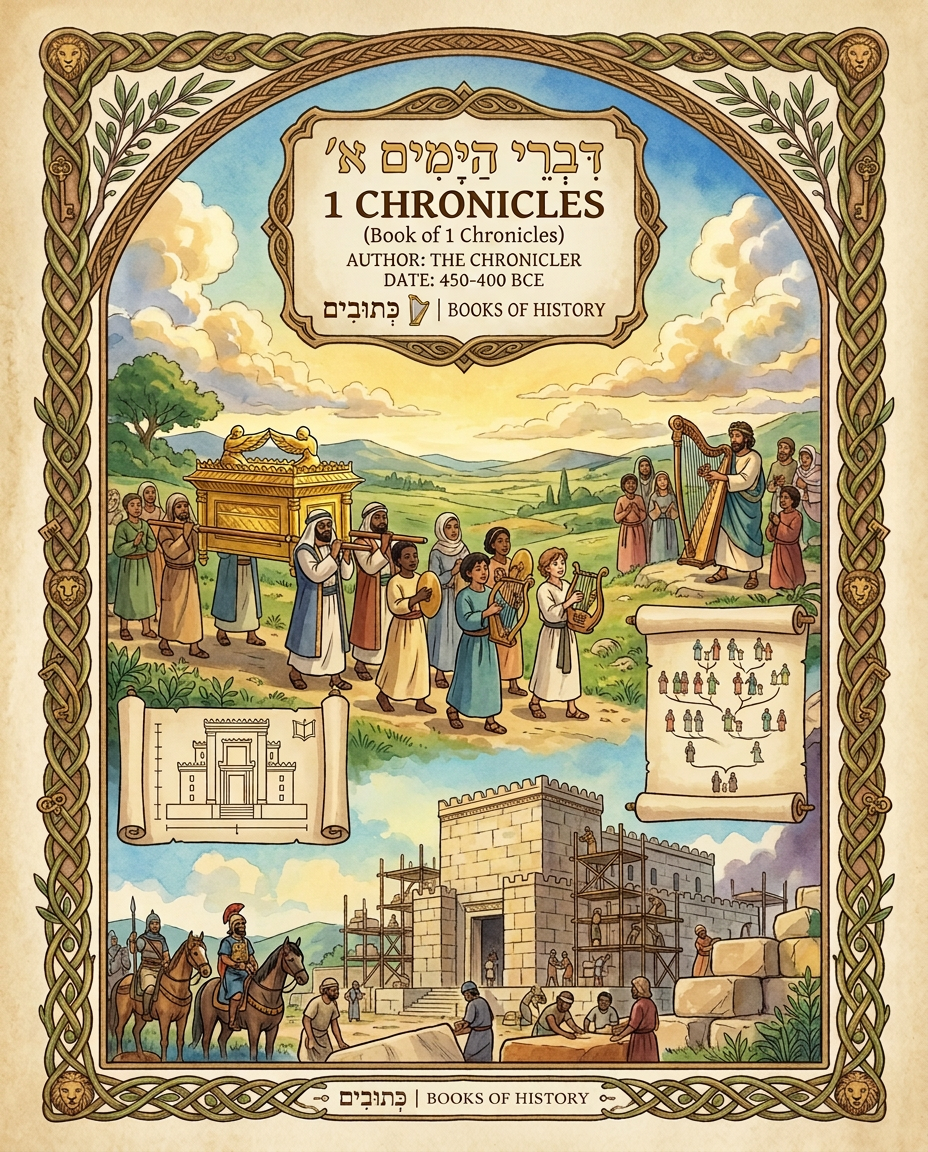
\includepdf[pages=1, fitpaper=false, width=\paperwidth, height=\paperheight, , keepaspectratio=false]{images/divider2/1_chronicles_2.png}

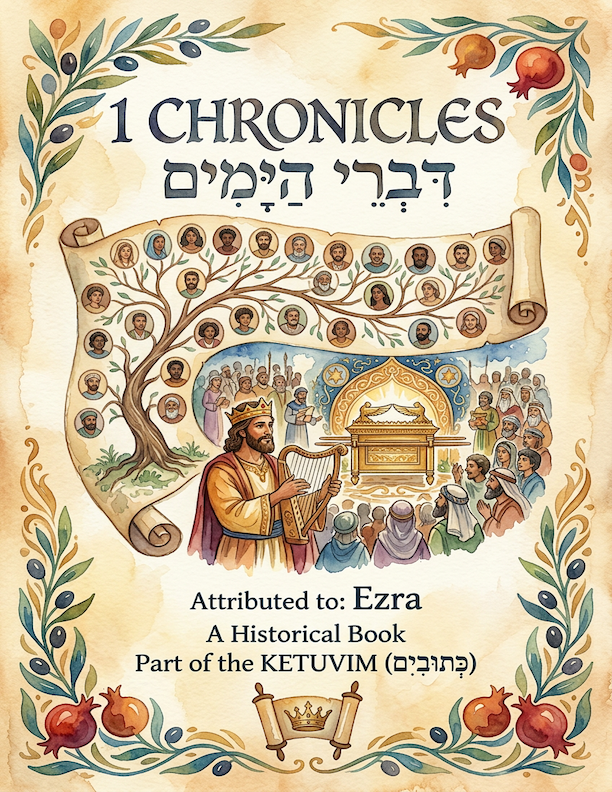
\includepdf[pages=1, fitpaper=false, width=\paperwidth, height=\paperheight, , keepaspectratio=false]{images/divider1/1_chronicles.png}


\includepdf[pages=1, fitpaper=false, width=\paperwidth, height=\paperheight, , keepaspectratio=false]{images/8.5x11-Dot-Grid.png}

\includepdf[pages=1, fitpaper=false, width=\paperwidth, height=\paperheight, , keepaspectratio=false]{images/8.5x11-Dot-Grid.png}


\mybook{1 Chronicles}
\vspace{-1.36in}

\mychapter{} \myverse*{}Adam, Seth, Enosh,
\myverse{}Kenan, Mahalalel, Jared,
\myverse{}Enoch, Methuselah, Lamech,
\myverse{}Noah, Shem, Ham, and Japheth.

\myverse{}The sons of Japheth: Gomer, Magog, Madai, Javan, Tubal, Meshech,
and Tiras.
\myverse{}The sons of Gomer: Ashkenaz, Diphath, and Togarmah.
\myverse{}The sons of Javan: Elishah, Tarshish, Kittim, and Rodanim.

\myverse{}The sons of Ham: Cush, Mizraim, Put, and Canaan.
\myverse{}The sons of Cush: Seba, Havilah, Sabta, Raama, Sabteca. The sons of Raamah:
Sheba and Dedan.
\myverse{}Cush became the father of Nimrod. He began to be a mighty one on the earth.
\myverse{}Mizraim became the father of Ludim, Anamim, Lehabim, Naphtuhim,
\myverse{}Pathrusim, Casluhim (where the Philistines came from), and Caphtorim.
\myverse{}Canaan became the father of Sidon his firstborn, Heth,
\myverse{}the Jebusite, the Amorite, the Girgashite,
\myverse{}the Hivite, the Arkite, the Sinite,
\myverse{}the Arvadite, the Zemarite, and the Hamathite.

\myverse{}The sons of Shem: Elam, Asshur, Arpachshad, Lud, Aram, Uz, Hul,
Gether, and Meshech.
\myverse{}Arpachshad became the father of Shelah, and Shelah became the father of Eber.
\myverse{}To Eber were born two sons: the name of the one was Peleg, for in his days
the earth was divided; and his brother’s name was Joktan.
\myverse{}Joktan became the father of Almodad, Sheleph, Hazarmaveth, Jerah,
\myverse{}Hadoram, Uzal, Diklah,
\myverse{}Ebal, Abimael, Sheba,
\myverse{}Ophir, Havilah, and Jobab. All these were the sons of Joktan.
\myverse{}Shem, Arpachshad, Shelah,
\myverse{}Eber, Peleg, Reu,
\myverse{}Serug, Nahor, Terah,
\myverse{}Abram (also called Abraham).

\myverse{}The sons of Abraham: Isaac and Ishmael.
\myverse{}These are their generations: the firstborn of Ishmael, Nebaioth; then Kedar,
Adbeel, Mibsam,
\myverse{}Mishma, Dumah, Massa, Hadad, Tema,
\myverse{}Jetur, Naphish, and Kedemah. These are the sons of Ishmael.

\myverse{}The sons of Keturah, Abraham’s concubine: she bore Zimran, Jokshan,
Medan, Midian, Ishbak, and Shuah. The sons of Jokshan: Sheba and Dedan.
\myverse{}The sons of Midian: Efah, Epher, Hanoch, Abida, and Eldaah. All these were
the sons of Keturah.

\myverse{}Abraham became the father of Isaac. The sons of Isaac: Esau and
Israel.
\myverse{}The sons of Esau: Eliphaz, Reuel, Jeush, Jalam, and Korah.
\myverse{}The sons of Eliphaz: Teman, Omar, Zephi, Gatam, Kenaz, Timna, and Amalek.
\myverse{}The sons of Reuel: Nahath, Zerah, Shammah, and Mizzah.

\myverse{}The sons of Seir: Lotan, Shobal, Zibeon, Anah, Dishon, Ezer,
and Dishan.
\myverse{}The sons of Lotan: Hori and Homam; and Timna was Lotan’s sister.
\myverse{}The sons of Shobal: Alian, Manahath, Ebal, Shephi, and Onam. The sons of Zibeon:
Aiah and Anah.
\myverse{}The son of Anah: Dishon. The sons of Dishon: Hamran, Eshban, Ithran, and Cheran.
\myverse{}The sons of Ezer: Bilhan, Zaavan, and Jaakan. The sons of Dishan: Uz and Aran.

\myverse{}Now these are the kings who reigned in the land of Edom, before
any king reigned over the children of Israel: Bela the son of Beor; and the name of his city was Dinhabah.
\myverse{}Bela died, and Jobab the son of Zerah of Bozrah reigned in his place.
\myverse{}Jobab died, and Husham of the land of the Temanites reigned in his place.
\myverse{}Husham died, and Hadad the son of Bedad, who struck Midian in the field of
Moab, reigned in his place; and the name of his city was Avith.
\myverse{}Hadad died, and Samlah of Masrekah reigned in his place.
\myverse{}Samlah died, and Shaul of Rehoboth by the River reigned in his place.
\myverse{}Shaul died, and Baal Hanan the son of Achbor reigned in his place.
\myverse{}Baal Hanan died, and Hadad reigned in his place; and the name of his city
was Pai. His wife’s name was Mehetabel, the daughter of Matred, the daughter of Mezahab.
\myverse{}Then Hadad died. The chiefs of Edom were: chief Timna, chief Aliah, chief
Jetheth,
\myverse{}chief Oholibamah, chief Elah, chief Pinon,
\myverse{}chief Kenaz, chief Teman, chief Mibzar,
\myverse{}chief Magdiel, and chief Iram. These are the chiefs of Edom.


%1 CHRONICLES 2
\mychapter{} \myverse*{}These are the sons of Israel: Reuben, Simeon, Levi, Judah, Issachar,
Zebulun,
\myverse{}Dan, Joseph, Benjamin, Naphtali, Gad, and Asher.

\myverse{}The sons of Judah: Er, Onan, and Shelah, which three were born
to him of Shua’s daughter the Canaanitess. Er, Judah’s firstborn, was wicked in the LORD’s\footnote{2:3 When rendered in ALL CAPITAL LETTERS, “LORD” or “GOD” is the translation of God’s Proper Name.}
sight; and he killed him.
\myverse{}Tamar his daughter-in-law bore him Perez and Zerah. All the sons of Judah were
five.

\myverse{}The sons of Perez: Hezron and Hamul.
\myverse{}The sons of Zerah: Zimri, Ethan, Heman, Calcol, and Dara—five of them in all.
\myverse{}The son of Carmi: Achar, the troubler of Israel, who committed a trespass in
the devoted thing.
\myverse{}The son of Ethan: Azariah.

\myverse{}The sons also of Hezron, who were born to him: Jerahmeel, Ram,
and Chelubai.
\myverse{}Ram became the father of Amminadab, and Amminadab became the father of Nahshon,
prince of the children of Judah;
\myverse{}and Nahshon became the father of Salma, and Salma became the father of Boaz,
\myverse{}and Boaz became the father of Obed, and Obed became the father of Jesse;
\myverse{}and Jesse became the father of his firstborn Eliab, Abinadab the second, Shimea
the third,
\myverse{}Nethanel the fourth, Raddai the fifth,
\myverse{}Ozem the sixth, and David the seventh;
\myverse{}and their sisters were Zeruiah and Abigail. The sons of Zeruiah: Abishai,
Joab, and Asahel, three.
\myverse{}Abigail bore Amasa; and the father of Amasa was Jether the Ishmaelite.

\myverse{}Caleb the son of Hezron became the father of children by Azubah
his wife, and by Jerioth; and these were her sons: Jesher, Shobab, and Ardon.
\myverse{}Azubah died, and Caleb married Ephrath, who bore him Hur.
\myverse{}Hur became the father of Uri, and Uri became the father of Bezalel.

\myverse{}Afterward Hezron went in to the daughter of Machir the father
of Gilead, whom he took as wife when he was sixty years old; and she bore him Segub.
\myverse{}Segub became the father of Jair, who had twenty-three cities in the land of
Gilead.
\myverse{}Geshur and Aram took the towns of Jair from them, with Kenath, and its villages,
even sixty cities. All these were the sons of Machir the father of Gilead.
\myverse{}After Hezron died in Caleb Ephrathah, Abijah, Hezron’s wife, bore him Ashhur
the father of Tekoa.

\myverse{}The sons of Jerahmeel the firstborn of Hezron were Ram the firstborn,
Bunah, Oren, Ozem, and Ahijah.
\myverse{}Jerahmeel had another wife, whose name was Atarah. She was the mother of Onam.
\myverse{}The sons of Ram the firstborn of Jerahmeel were Maaz, Jamin, and Eker.
\myverse{}The sons of Onam were Shammai and Jada. The sons of Shammai: Nadab and Abishur.
\myverse{}The name of the wife of Abishur was Abihail; and she bore him Ahban and Molid.
\myverse{}The sons of Nadab: Seled and Appaim; but Seled died without children.
\myverse{}The son of Appaim: Ishi. The son of Ishi: Sheshan. The son of Sheshan: Ahlai.
\myverse{}The sons of Jada the brother of Shammai: Jether and Jonathan; and Jether died
without children.
\myverse{}The sons of Jonathan: Peleth and Zaza. These were the sons of Jerahmeel.
\myverse{}Now Sheshan had no sons, but only daughters. Sheshan had a servant, an Egyptian,
whose name was Jarha.
\myverse{}Sheshan gave his daughter to Jarha his servant as wife; and she bore him Attai.
\myverse{}Attai became the father of Nathan, and Nathan became the father of Zabad,
\myverse{}and Zabad became the father of Ephlal, and Ephlal became the father of Obed,
\myverse{}and Obed became the father of Jehu, and Jehu became the father of Azariah,
\myverse{}and Azariah became the father of Helez, and Helez became the father of Eleasah,
\myverse{}and Eleasah became the father of Sismai, and Sismai became the father of Shallum,
\myverse{}and Shallum became the father of Jekamiah, and Jekamiah became the father
of Elishama.

\myverse{}The sons of Caleb the brother of Jerahmeel were Mesha his firstborn,
who was the father of Ziph, and the sons of Mareshah the father of Hebron.
\myverse{}The sons of Hebron: Korah, Tappuah, Rekem, and Shema.
\myverse{}Shema became the father of Raham, the father of Jorkeam; and Rekem became
the father of Shammai.
\myverse{}The son of Shammai was Maon; and Maon was the father of Beth Zur.
\myverse{}Efah, Caleb’s concubine, bore Haran, Moza, and Gazez; and Haran became the
father of Gazez.
\myverse{}The sons of Jahdai: Regem, Jothan, Geshan, Pelet, Efah, and Shaaph.
\myverse{}Maacah, Caleb’s concubine, bore Sheber and Tirhanah.
\myverse{}She bore also Shaaph the father of Madmannah, Sheva the father of Machbena
and the father of Gibea; and the daughter of Caleb was Achsah.

\myverse{}These were the sons of Caleb, the son of Hur, the firstborn of
Ephrathah: Shobal the father of Kiriath Jearim,
\myverse{}Salma the father of Bethlehem, and Hareph the father of Beth Gader.
\myverse{}Shobal the father of Kiriath Jearim had sons: Haroeh, half of the Menuhoth.
\myverse{}The families of Kiriath Jearim: the Ithrites, the Puthites, the Shumathites,
and the Mishraites; from them came the Zorathites and the Eshtaolites.
\myverse{}The sons of Salma: Bethlehem, the Netophathites, Atroth Beth Joab, and half
of the Manahathites, the Zorites.
\myverse{}The families of scribes who lived at Jabez: the Tirathites, the Shimeathites,
and the Sucathites. These are the Kenites who came from Hammath, the father of the house of Rechab.


% 1 CHRONICLES 3
\mychapter{} \myverse*{}Now these were the sons of David, who were born to him in Hebron:
the firstborn, Amnon, of Ahinoam the Jezreelitess; the second, Daniel, of Abigail the Carmelitess;
\myverse{}the third, Absalom the son of Maacah the daughter of Talmai king of Geshur;
the fourth, Adonijah the son of Haggith;
\myverse{}the fifth, Shephatiah of Abital; the sixth, Ithream by Eglah his wife:
\myverse{}six were born to him in Hebron; and he reigned there seven years and six months.
He reigned thirty-three years in Jerusalem;
\myverse{}and these were born to him in Jerusalem: Shimea, Shobab, Nathan, and Solomon,
four, by Bathshua the daughter of Ammiel;
\myverse{}and Ibhar, Elishama, Eliphelet,
\myverse{}Nogah, Nepheg, Japhia,
\myverse{}Elishama, Eliada, and Eliphelet, nine.
\myverse{}All these were the sons of David, in addition to the sons of the concubines;
and Tamar was their sister.

\myverse{}Solomon’s son was Rehoboam, Abijah his son, Asa his son, Jehoshaphat
his son,
\myverse{}Joram his son, Ahaziah his son, Joash his son,
\myverse{}Amaziah his son, Azariah his son, Jotham his son,
\myverse{}Ahaz his son, Hezekiah his son, Manasseh his son,
\myverse{}Amon his son, and Josiah his son.
\myverse{}The sons of Josiah: the firstborn Yochanan, the second Jehoiakim, the third
Zedekiah, and the fourth Shallum.
\myverse{}The sons of Jehoiakim: Jeconiah his son, and Zedekiah his son.
\myverse{}The sons of Jeconiah, the captive: Shealtiel his son,
\myverse{}Malchiram, Pedaiah, Shenazzar, Jekamiah, Hoshama, and Nedabiah.
\myverse{}The sons of Pedaiah: Zerubbabel and Shimei. The sons of Zerubbabel: Meshullam
and Hananiah; and Shelomith was their sister;
\myverse{}and Hashubah, Ohel, Berechiah, Hasadiah, and Jushab Hesed, five.
\myverse{}The sons of Hananiah: Pelatiah and Jeshaiah; the sons of Rephaiah, the sons
of Arnan, the sons of Obadiah, the sons of Shecaniah.
\myverse{}The son of Shecaniah: Shemaiah. The sons of Shemaiah: Hattush, Igal, Bariah,
Neariah, and Shaphat, six.
\myverse{}The sons of Neariah: Elioenai, Hizkiah, and Azrikam, three.
\myverse{}The sons of Elioenai: Hodaviah, Eliashib, Pelaiah, Akkub, Yochanan, Delaiah,
and Anani, seven.


% 1 CHRONICLES 4
\mychapter{} \myverse*{}The sons of Judah: Perez, Hezron, Carmi, Hur, and Shobal.
\myverse{}Reaiah the son of Shobal became the father of Jahath; and Jahath became the
father of Ahumai and Lahad. These are the families of the Zorathites.
\myverse{}These were the sons of the father of Etam: Jezreel, Ishma, and Idbash. The name
of their sister was Hazzelelponi.
\myverse{}Penuel was the father of Gedor and Ezer the father of Hushah. These are the
sons of Hur, the firstborn of Ephrathah, the father of Bethlehem.
\myverse{}Ashhur the father of Tekoa had two wives, Helah and Naarah.
\myverse{}Naarah bore him Ahuzzam, Hepher, Temeni, and Haahashtari. These were the sons
of Naarah.
\myverse{}The sons of Helah were Zereth, Izhar, and Ethnan.
\myverse{}Hakkoz became the father of Anub, Zobebah, and the families of Aharhel the son
of Harum.

\myverse{}Jabez was more honorable than his brothers. His mother named him
Jabez,\footnote{4:9 “Jabez” sounds similar to the Hebrew word for “pain”.} saying, “Because I bore him with
sorrow.”

\myverse{}Jabez called on the God\footnote{4:10 The Hebrew word rendered “God” is “אֱלֹהִ֑ים” (Elohim).} of Israel, saying,
“Oh that you would bless me indeed, and enlarge my border! May your hand be with me, and may you keep
me from evil, that I may not cause pain!”

God granted him that which he requested.

\myverse{}Chelub the brother of Shuhah became the father of Mehir, who
was the father of Eshton.
\myverse{}Eshton became the father of Beth Rapha, Paseah, and Tehinnah the father of
Ir Nahash. These are the men of Recah.
\myverse{}The sons of Kenaz: Othniel and Seraiah. The sons of Othniel: Hathath.\footnote{4:13 Greek and Vulgate add “and Meonothai”}
\myverse{}Meonothai became the father of Ophrah: and Seraiah became the father of Joab
the father of Ge Harashim, for they were craftsmen.
\myverse{}The sons of Caleb the son of Jephunneh: Iru, Elah, and Naam. The son of Elah:
Kenaz.
\myverse{}The sons of Jehallelel: Ziph, Ziphah, Tiria, and Asarel.
\myverse{}The sons of Ezrah: Jether, Mered, Epher, and Jalon; and Mered’s wife bore
Miriam, Shammai, and Ishbah the father of Eshtemoa.
\myverse{}His wife Yehudiyah bore Jered the father of Gedor, Heber the father of Soco,
and Jekuthiel the father of Zanoah. These are the sons of Bithiah the daughter of Pharaoh, whom Mered
took.
\myverse{}The sons of the wife of Hodiah, the sister of Naham, were the fathers of Keilah
the Garmite and Eshtemoa the Maacathite.
\myverse{}The sons of Shimon: Amnon, Rinnah, Ben Hanan, and Tilon. The sons of Ishi:
Zoheth, and Ben Zoheth.
\myverse{}The sons of Shelah the son of Judah: Er the father of Lecah, Laadah the father
of Mareshah, and the families of the house of those who worked fine linen, of the house of Ashbea;
\myverse{}and Jokim, and the men of Cozeba, and Joash, and Saraph, who had dominion
in Moab, and Jashubilehem. These records are ancient.
\myverse{}These were the potters, and the inhabitants of Netaim and Gederah; they lived
there with the king for his work.

\myverse{}The sons of Simeon: Nemuel, Jamin, Jarib, Zerah, Shaul;
\myverse{}Shallum his son, Mibsam his son, and Mishma his son.
\myverse{}The sons of Mishma: Hammuel his son, Zaccur his son, Shimei his son.
\myverse{}Shimei had sixteen sons and six daughters; but his brothers didn’t have many
children, and all their family didn’t multiply like the children of Judah.
\myverse{}They lived at Beersheba, Moladah, Hazarshual,
\myverse{}at Bilhah, at Ezem, at Tolad,
\myverse{}at Bethuel, at Hormah, at Ziklag,
\myverse{}at Beth Marcaboth, Hazar Susim, at Beth Biri, and at Shaaraim. These were
their cities until David’s reign.
\myverse{}Their villages were Etam, Ain, Rimmon, Tochen, and Ashan, five cities;
\myverse{}and all their villages that were around the same cities, as far as Baal. These
were their settlements, and they kept their genealogy.
\myverse{}Meshobab, Jamlech, Joshah the son of Amaziah,
\myverse{}Joel, Jehu the son of Joshibiah, the son of Seraiah, the son of Asiel,
\myverse{}Elioenai, Jaakobah, Jeshohaiah, Asaiah, Adiel, Jesimiel, Benaiah,
\myverse{}and Ziza the son of Shiphi, the son of Allon, the son of Jedaiah, the son
of Shimri, the son of Shemaiah—
\myverse{}these mentioned by name were princes in their families. Their fathers’ houses
increased greatly.

\myverse{}They went to the entrance of Gedor, even to the east side of
the valley, to seek pasture for their flocks.
\myverse{}They found rich, good pasture, and the land was wide, and quiet, and peaceful,
for those who lived there before were descended from Ham.
\myverse{}These written by name came in the days of Hezekiah king of Judah, and struck
their tents and the Meunim who were found there; and they destroyed them utterly to this day, and lived
in their place, because there was pasture there for their flocks.
\myverse{}Some of them, even of the sons of Simeon, five hundred men, went to Mount
Seir, having for their captains Pelatiah, Neariah, Rephaiah, and Uzziel, the sons of Ishi.
\myverse{}They struck the remnant of the Amalekites who escaped, and have lived there
to this day.


% 1 CHRONICLES 5
\mychapter{} \myverse*{}The sons of Reuben the firstborn of Israel (for he was the firstborn,
but because he defiled his father’s couch, his birthright was given to the sons of Joseph the son of Israel;
and the genealogy is not to be listed according to the birthright.
\myverse{}For Judah prevailed above his brothers, and from him came the prince; but the
birthright was Joseph’s)—
\myverse{}the sons of Reuben the firstborn of Israel: Hanoch, Pallu, Hezron, and Carmi.
\myverse{}The sons of Joel: Shemaiah his son, Gog his son, Shimei his son,
\myverse{}Micah his son, Reaiah his son, Baal his son,
\myverse{}and Beerah his son, whom Tilgath Pilneser king of Assyria carried away captive.
He was prince of the Reubenites.
\myverse{}His brothers by their families, when the genealogy of their generations was
listed: the chief, Jeiel, and Zechariah,
\myverse{}and Bela the son of Azaz, the son of Shema, the son of Joel, who lived in Aroer,
even to Nebo and Baal Meon;
\myverse{}and he lived eastward even to the entrance of the wilderness from the river
Euphrates, because their livestock were multiplied in the land of Gilead.

\myverse{}In the days of Saul, they made war with the Hagrites, who fell
by their hand; and they lived in their tents throughout all the land east of Gilead.

\myverse{}The sons of Gad lived beside them in the land of Bashan to Salecah:
\myverse{}Joel the chief, Shapham the second, Janai, and Shaphat in Bashan.
\myverse{}Their brothers of their fathers’ houses: Michael, Meshullam, Sheba, Jorai,
Jacan, Zia, and Eber, seven.
\myverse{}These were the sons of Abihail, the son of Huri, the son of Jaroah, the son
of Gilead, the son of Michael, the son of Jeshishai, the son of Jahdo, the son of Buz;
\myverse{}Ahi the son of Abdiel, the son of Guni, chief of their fathers’ houses.
\myverse{}They lived in Gilead in Bashan and in its towns, and in all the pasture lands
of Sharon as far as their borders.
\myverse{}All these were listed by genealogies in the days of Jotham king of Judah,
and in the days of Jeroboam king of Israel.

\myverse{}The sons of Reuben, the Gadites, and the half-tribe of Manasseh,
of valiant men, men able to bear buckler and sword, able to shoot with bow, and skillful in war, were
forty-four thousand seven hundred sixty that were able to go out to war.
\myverse{}They made war with the Hagrites, with Jetur, and Naphish, and Nodab.
\myverse{}They were helped against them, and the Hagrites were delivered into their
hand, and all who were with them; for they cried to God in the battle, and he answered them because they
put their trust in him.
\myverse{}They took away their livestock: of their camels fifty thousand, and of sheep
two hundred fifty thousand, and of donkeys two thousand, and of men one hundred thousand.
\myverse{}For many fell slain, because the war was of God. They lived in their place
until the captivity.

\myverse{}The children of the half-tribe of Manasseh lived in the land.
They increased from Bashan to Baal Hermon, Senir, and Mount Hermon.
\myverse{}These were the heads of their fathers’ houses: Epher, Ishi, Eliel, Azriel,
Jeremiah, Hodaviah, and Jahdiel—mighty men of valor, famous men, heads of their fathers’ houses.
\myverse{}They trespassed against the God of their fathers, and played the prostitute
after the gods of the peoples of the land whom God destroyed before them.
\myverse{}So the God of Israel stirred up the spirit of Pul king of Assyria, and the
spirit of Tilgath Pilneser king of Assyria, and he carried away the Reubenites, the Gadites, and the half-tribe
of Manasseh, and brought them to Halah, Habor, Hara, and to the river of Gozan, to this day.


% 1 CHRONICLES 6
\mychapter{} \myverse*{}The sons of Levi: Gershon, Kohath, and Merari.
\myverse{}The sons of Kohath: Amram, Izhar, Hebron, and Uzziel.
\myverse{}The children of Amram: Aaron, Moses, and Miriam. The sons of Aaron: Nadab, Abihu,
Eleazar, and Ithamar.
\myverse{}Eleazar became the father of Phinehas, Phinehas became the father of Abishua,
\myverse{}Abishua became the father of Bukki. Bukki became the father of Uzzi.
\myverse{}Uzzi became the father of Zerahiah. Zerahiah became the father of Meraioth.
\myverse{}Meraioth became the father of Amariah. Amariah became the father of Ahitub.
\myverse{}Ahitub became the father of Zadok. Zadok became the father of Ahimaaz.
\myverse{}Ahimaaz became the father of Azariah. Azariah became the father of Yochanan.
\myverse{}Yochanan became the father of Azariah, who executed the priest’s office in
the house that Solomon built in Jerusalem.
\myverse{}Azariah became the father of Amariah. Amariah became the father of Ahitub.
\myverse{}Ahitub became the father of Zadok. Zadok became the father of Shallum.
\myverse{}Shallum became the father of Hilkiah. Hilkiah became the father of Azariah.
\myverse{}Azariah became the father of Seraiah. Seraiah became the father of Jehozadak.
\myverse{}Jehozadak went into captivity when the LORD carried Judah and Jerusalem away
by the hand of Nebuchadnezzar.

\myverse{}The sons of Levi: Gershom, Kohath, and Merari.
\myverse{}These are the names of the sons of Gershom: Libni and Shimei.
\myverse{}The sons of Kohath were Amram, Izhar, Hebron, and Uzziel.
\myverse{}The sons of Merari: Mahli and Mushi. These are the families of the Levites
according to their fathers’ households.
\myverse{}Of Gershom: Libni his son, Jahath his son, Zimmah his son,
\myverse{}Joah his son, Iddo his son, Zerah his son, and Jeatherai his son.
\myverse{}The sons of Kohath: Amminadab his son, Korah his son, Assir his son,
\myverse{}Elkanah his son, Ebiasaph his son, Assir his son,
\myverse{}Tahath his son, Uriel his son, Uzziah his son, and Shaul his son.
\myverse{}The sons of Elkanah: Amasai and Ahimoth.
\myverse{}As for Elkanah, the sons of Elkanah: Zophai his son, Nahath his son,
\myverse{}Eliab his son, Jeroham his son, and Elkanah his son.
\myverse{}The sons of Samuel: the firstborn, Joel, and the second, Abijah.
\myverse{}The sons of Merari: Mahli, Libni his son, Shimei his son, Uzzah his son,
\myverse{}Shimea his son, Haggiah his son, Asaiah his son.

\myverse{}These are they whom David set over the service of song in the
LORD’s house after the ark came to rest there.
\myverse{}They ministered with song before the tabernacle of the Tent of Meeting until
Solomon had built the LORD’s house in Jerusalem. They performed the duties of their office according to
their order.
\myverse{}These are those who served, and their sons. Of the sons of the Kohathites:
Heman the singer, the son of Joel, the son of Samuel,
\myverse{}the son of Elkanah, the son of Jeroham, the son of Eliel, the son of Toah,
\myverse{}the son of Zuph, the son of Elkanah, the son of Mahath, the son of Amasai,
\myverse{}the son of Elkanah, the son of Joel, the son of Azariah, the son of Zephaniah,
\myverse{}the son of Tahath, the son of Assir, the son of Ebiasaph, the son of Korah,
\myverse{}the son of Izhar, the son of Kohath, the son of Levi, the son of Israel.
\myverse{}His brother Asaph, who stood on his right hand, even Asaph the son of Berechiah,
the son of Shimea,
\myverse{}the son of Michael, the son of Baaseiah, the son of Malchijah,
\myverse{}the son of Ethni, the son of Zerah, the son of Adaiah,
\myverse{}the son of Ethan, the son of Zimmah, the son of Shimei,
\myverse{}the son of Jahath, the son of Gershom, the son of Levi.
\myverse{}On the left hand their brothers the sons of Merari: Ethan the son of Kishi,
the son of Abdi, the son of Malluch,
\myverse{}the son of Hashabiah, the son of Amaziah, the son of Hilkiah,
\myverse{}the son of Amzi, the son of Bani, the son of Shemer,
\myverse{}the son of Mahli, the son of Mushi, the son of Merari, the son of Levi.
\myverse{}Their brothers the Levites were appointed for all the service of the tabernacle
of God’s house.
\myverse{}But Aaron and his sons offered on the altar of burnt offering, and on the
altar of incense, for all the work of the most holy place, and to make atonement for Israel, according
to all that Moses the servant of God had commanded.

\myverse{}These are the sons of Aaron: Eleazar his son, Phinehas his son,
Abishua his son,
\myverse{}Bukki his son, Uzzi his son, Zerahiah his son,
\myverse{}Meraioth his son, Amariah his son, Ahitub his son,
\myverse{}Zadok his son, and Ahimaaz his son.
\myverse{}Now these are their dwelling places according to their encampments in their
borders: to the sons of Aaron, of the families of the Kohathites (for theirs was the first lot),
\myverse{}to them they gave Hebron in the land of Judah, and its pasture lands around
it;
\myverse{}but the fields of the city and its villages, they gave to Caleb the son of
Jephunneh.
\myverse{}To the sons of Aaron they gave the cities of refuge, Hebron, Libnah also with
its pasture lands, Jattir, Eshtemoa with its pasture lands,
\myverse{}Hilen with its pasture lands, Debir with its pasture lands,
\myverse{}Ashan with its pasture lands, and Beth Shemesh with its pasture lands;
\myverse{}and out of the tribe of Benjamin, Geba with its pasture lands, Allemeth with
its pasture lands, and Anathoth with its pasture lands. All their cities throughout their families were
thirteen cities.

\myverse{}To the rest of the sons of Kohath were given by lot, out of the
family of the tribe, out of the half-tribe, the half of Manasseh, ten cities.
\myverse{}To the sons of Gershom, according to their families, out of the tribe of Issachar,
and out of the tribe of Asher, and out of the tribe of Naphtali, and out of the tribe of Manasseh in Bashan,
thirteen cities.
\myverse{}To the sons of Merari were given by lot, according to their families, out
of the tribe of Reuben, and out of the tribe of Gad, and out of the tribe of Zebulun, twelve cities.
\myverse{}The children of Israel gave to the Levites the cities with their pasture lands.
\myverse{}They gave by lot out of the tribe of the children of Judah, and out of the
tribe of the children of Simeon, and out of the tribe of the children of Benjamin, these cities which
are mentioned by name.

\myverse{}Some of the families of the sons of Kohath had cities of their
borders out of the tribe of Ephraim.
\myverse{}They gave to them the cities of refuge, Shechem in the hill country of Ephraim
with its pasture lands and Gezer with its pasture lands,
\myverse{}Jokmeam with its pasture lands, Beth Horon with its pasture lands,
\myverse{}Aijalon with its pasture lands, Gath Rimmon with its pasture lands;
\myverse{}and out of the half-tribe of Manasseh, Aner with its pasture lands, and Bileam
with its pasture lands, for the rest of the family of the sons of Kohath.

\myverse{}To the sons of Gershom were given, out of the family of the half-tribe
of Manasseh, Golan in Bashan with its pasture lands, and Ashtaroth with its pasture lands;
\myverse{}and out of the tribe of Issachar, Kedesh with its pasture lands, Daberath
with its pasture lands,
\myverse{}Ramoth with its pasture lands, and Anem with its pasture lands;
\myverse{}and out of the tribe of Asher, Mashal with its pasture lands, Abdon with its
pasture lands,
\myverse{}Hukok with its pasture lands, and Rehob with its pasture lands;
\myverse{}and out of the tribe of Naphtali, Kedesh in Galilee with its pasture lands,
Hammon with its pasture lands, and Kiriathaim with its pasture lands.

\myverse{}To the rest of the Levites, the sons of Merari, were given, out
of the tribe of Zebulun, Rimmono with its pasture lands, and Tabor with its pasture lands;
\myverse{}and beyond the Jordan at Jericho, on the east side of the Jordan, were given
them out of the tribe of Reuben: Bezer in the wilderness with its pasture lands, Jahzah with its pasture
lands,
\myverse{}Kedemoth with its pasture lands, and Mephaath with its pasture lands;
\myverse{}and out of the tribe of Gad, Ramoth in Gilead with its pasture lands, Mahanaim
with its pasture lands,
\myverse{}Heshbon with its pasture lands, and Jazer with its pasture lands.


%1 CHRONICLES 7
\mychapter{} \myverse*{}Of the sons of Issachar: Tola, Puah, Jashub, and Shimron, four.
\myverse{}The sons of Tola: Uzzi, Rephaiah, Jeriel, Jahmai, Ibsam, and Shemuel, heads
of their fathers’ houses, of Tola; mighty men of valor in their generations. Their number in the days
of David was twenty-two thousand six hundred.
\myverse{}The son of Uzzi: Izrahiah. The sons of Izrahiah: Michael, Obadiah, Joel, and
Isshiah, five; all of them chief men.
\myverse{}With them, by their generations, after their fathers’ houses, were bands of
the army for war, thirty-six thousand; for they had many wives and sons.
\myverse{}Their brothers among all the families of Issachar, mighty men of valor, listed
in all by genealogy, were eighty-seven thousand.

\myverse{}The sons of Benjamin: Bela, Becher, and Jediael, three.
\myverse{}The sons of Bela: Ezbon, Uzzi, Uzziel, Jerimoth, and Iri, five; heads of fathers’
houses, mighty men of valor; and they were listed by genealogy twenty-two thousand thirty-four.
\myverse{}The sons of Becher: Zemirah, Joash, Eliezer, Elioenai, Omri, Jeremoth, Abijah,
Anathoth, and Alemeth. All these were the sons of Becher.
\myverse{}They were listed by genealogy, after their generations, heads of their fathers’
houses, mighty men of valor, twenty thousand two hundred.
\myverse{}The son of Jediael: Bilhan. The sons of Bilhan: Jeush, Benjamin, Ehud, Chenaanah,
Zethan, Tarshish, and Ahishahar.
\myverse{}All these were sons of Jediael, according to the heads of their fathers’ households,
mighty men of valor, seventeen thousand two hundred, who were able to go out in the army for war.
\myverse{}So were Shuppim, Huppim, the sons of Ir, Hushim, and the sons of Aher.

\myverse{}The sons of Naphtali: Jahziel, Guni, Jezer, Shallum, and the
sons of Bilhah.

\myverse{}The sons of Manasseh: Asriel, whom his concubine the Aramitess
bore. She bore Machir the father of Gilead.
\myverse{}Machir took a wife of Huppim and Shuppim, whose sister’s name was Maacah.
The name of the second was Zelophehad; and Zelophehad had daughters.
\myverse{}Maacah the wife of Machir bore a son, and she named him Peresh. The name of
his brother was Sheresh; and his sons were Ulam and Rakem.
\myverse{}The sons of Ulam: Bedan. These were the sons of Gilead the son of Machir,
the son of Manasseh.
\myverse{}His sister Hammolecheth bore Ishhod, Abiezer, and Mahlah.
\myverse{}The sons of Shemida were Ahian, Shechem, Likhi, and Aniam.

\myverse{}The sons of Ephraim: Shuthelah, Bered his son, Tahath his son,
Eleadah his son, Tahath his son,
\myverse{}Zabad his son, Shuthelah his son, Ezer, and Elead, whom the men of Gath who
were born in the land killed, because they came down to take away their livestock.
\myverse{}Ephraim their father mourned many days, and his brothers came to comfort him.
\myverse{}He went in to his wife, and she conceived and bore a son, and he named him
Beriah,\footnote{7:23 “Beriah” is similar to the Hebrew word for “misfortune”.} because there was trouble with
his house.
\myverse{}His daughter was Sheerah, who built Beth Horon the lower and the upper, and
Uzzen Sheerah.
\myverse{}Rephah was his son, Resheph his son, Telah his son, Tahan his son,
\myverse{}Ladan his son, Ammihud his son, Elishama his son,
\myverse{}Nun his son, and Joshua his son.
\myverse{}Their possessions and settlements were Bethel and its towns, and eastward
Naaran, and westward Gezer with its towns; Shechem also and its towns, to Azzah and its towns;
\myverse{}and by the borders of the children of Manasseh, Beth Shean and its towns,
Taanach and its towns, Megiddo and its towns, and Dor and its towns. The children of Joseph the son of
Israel lived in these.

\myverse{}The sons of Asher: Imnah, Ishvah, Ishvi, and Beriah. Serah was
their sister.
\myverse{}The sons of Beriah: Heber and Malchiel, who was the father of Birzaith.
\myverse{}Heber became the father of Japhlet, Shomer, Hotham, and Shua their sister.
\myverse{}The sons of Japhlet: Pasach, Bimhal, and Ashvath. These are the children of
Japhlet.
\myverse{}The sons of Shemer: Ahi, Rohgah, Jehubbah, and Aram.
\myverse{}The sons of Helem his brother: Zophah, Imna, Shelesh, and Amal.
\myverse{}The sons of Zophah: Suah, Harnepher, Shual, Beri, Imrah,
\myverse{}Bezer, Hod, Shamma, Shilshah, Ithran, and Beera.
\myverse{}The sons of Jether: Jephunneh, Pispa, and Ara.
\myverse{}The sons of Ulla: Arah, Hanniel, and Rizia.
\myverse{}All these were the children of Asher, heads of the fathers’ houses, choice
and mighty men of valor, chief of the princes. The number of them listed by genealogy for service in war
was twenty-six thousand men.


% 1 CHRONICLES 8
\mychapter{} \myverse*{}Benjamin became the father of Bela his firstborn, Ashbel the second,
Aharah the third,
\myverse{}Nohah the fourth, and Rapha the fifth.
\myverse{}Bela had sons: Addar, Gera, Abihud,
\myverse{}Abishua, Naaman, Ahoah,
\myverse{}Gera, Shephuphan, and Huram.
\myverse{}These are the sons of Ehud. These are the heads of fathers’ households of the
inhabitants of Geba, who were carried captive to Manahath:
\myverse{}Naaman, Ahijah, and Gera, who carried them captive; and he became the father
of Uzza and Ahihud.

\myverse{}Shaharaim became the father of children in the field of Moab, after
he had sent them away. Hushim and Baara were his wives.
\myverse{}By Hodesh his wife, he became the father of Jobab, Zibia, Mesha, Malcam,
\myverse{}Jeuz, Shachia, and Mirmah. These were his sons, heads of fathers’ households.
\myverse{}By Hushim, he became the father of Abitub and Elpaal.
\myverse{}The sons of Elpaal: Eber, Misham, and Shemed, who built Ono and Lod, with
its towns;
\myverse{}and Beriah and Shema, who were heads of fathers’ households of the inhabitants
of Aijalon, who put to flight the inhabitants of Gath;
\myverse{}and Ahio, Shashak, Jeremoth,
\myverse{}Zebadiah, Arad, Eder,
\myverse{}Michael, Ishpah, Joha, the sons of Beriah,
\myverse{}Zebadiah, Meshullam, Hizki, Heber,
\myverse{}Ishmerai, Izliah, Jobab, the sons of Elpaal,
\myverse{}Jakim, Zichri, Zabdi,
\myverse{}Elienai, Zillethai, Eliel,
\myverse{}Adaiah, Beraiah, Shimrath, the sons of Shimei,
\myverse{}Ishpan, Eber, Eliel,
\myverse{}Abdon, Zichri, Hanan,
\myverse{}Hananiah, Elam, Anthothijah,
\myverse{}Iphdeiah, Penuel, the sons of Shashak,
\myverse{}Shamsherai, Shehariah, Athaliah,
\myverse{}Jaareshiah, Elijah, Zichri, and the sons of Jeroham.
\myverse{}These were heads of fathers’ households throughout their generations, chief
men. These lived in Jerusalem.

\myverse{}The father of Gibeon, whose wife’s name was Maacah, lived in
Gibeon
\myverse{}with his firstborn son Abdon, Zur, Kish, Baal, Nadab,
\myverse{}Gedor, Ahio, Zecher,
\myverse{}and Mikloth, who became the father of Shimeah. They also lived with their
families in Jerusalem, near their relatives.
\myverse{}Ner became the father of Kish. Kish became the father of Saul. Saul became
the father of Jonathan, Malchishua, Abinadab, and Eshbaal.
\myverse{}The son of Jonathan was Merib-baal. Merib-baal became the father of Micah.
\myverse{}The sons of Micah: Pithon, Melech, Tarea, and Ahaz.
\myverse{}Ahaz became the father of Jehoaddah. Jehoaddah became the father of Alemeth,
Azmaveth, and Zimri. Zimri became the father of Moza.
\myverse{}Moza became the father of Binea. Raphah was his son, Eleasah his son, and
Azel his son.
\myverse{}Azel had six sons, whose names are these: Azrikam, Bocheru, Ishmael, Sheariah,
Obadiah, and Hanan. All these were the sons of Azel.
\myverse{}The sons of Eshek his brother: Ulam his firstborn, Jeush the second, and Eliphelet
the third.
\myverse{}The sons of Ulam were mighty men of valor, archers, and had many sons, and
grandsons, one hundred fifty. All these were of the sons of Benjamin.


%1 CHRONICLE 9
\mychapter{} \myverse*{}So all Israel were listed by genealogies; and behold,\footnote{9:1 “Behold”, from “הִנֵּה”, means look at, take notice, observe, see, or gaze at. It is
	often used as an interjection.} they are written in the book of the kings of Israel. Judah was
carried away captive to Babylon for their disobedience.
\myverse{}Now the first inhabitants who lived in their possessions in their cities were
Israel, the priests, the Levites, and the temple servants.
\myverse{}In Jerusalem, there lived of the children of Judah, of the children of Benjamin,
and of the children of Ephraim and Manasseh:
\myverse{}Uthai the son of Ammihud, the son of Omri, the son of Imri, the son of Bani,
of the children of Perez the son of Judah.
\myverse{}Of the Shilonites: Asaiah the firstborn and his sons.
\myverse{}Of the sons of Zerah: Jeuel and their brothers, six hundred ninety.
\myverse{}Of the sons of Benjamin: Sallu the son of Meshullam, the son of Hodaviah, the
son of Hassenuah;
\myverse{}and Ibneiah the son of Jeroham, and Elah the son of Uzzi, the son of Michri;
and Meshullam the son of Shephatiah, the son of Reuel, the son of Ibnijah;
\myverse{}and their brothers, according to their generations, nine hundred fifty-six.
All these men were heads of fathers’ households by their fathers’ houses.

\myverse{}Of the priests: Jedaiah, Jehoiarib, Jachin,
\myverse{}and Azariah the son of Hilkiah, the son of Meshullam, the son of Zadok, the
son of Meraioth, the son of Ahitub, the ruler of God’s house;
\myverse{}and Adaiah the son of Jeroham, the son of Pashhur, the son of Malchijah; and
Maasai the son of Adiel, the son of Jahzerah, the son of Meshullam, the son of Meshillemith, the son of
Immer;
\myverse{}and their brothers, heads of their fathers’ houses, one thousand seven hundred
sixty; they were very able men for the work of the service of God’s house.

\myverse{}Of the Levites: Shemaiah the son of Hasshub, the son of Azrikam,
the son of Hashabiah, of the sons of Merari;
\myverse{}and Bakbakkar, Heresh, Galal, and Mattaniah the son of Mica, the son of Zichri,
the son of Asaph,
\myverse{}and Obadiah the son of Shemaiah, the son of Galal, the son of Jeduthun; and
Berechiah the son of Asa, the son of Elkanah, who lived in the villages of the Netophathites.

\myverse{}The gatekeepers: Shallum, Akkub, Talmon, Ahiman, and their brothers
(Shallum was the chief),
\myverse{}who previously served in the king’s gate eastward. They were the gatekeepers
for the camp of the children of Levi.
\myverse{}Shallum was the son of Kore, the son of Ebiasaph, the son of Korah, and his
brothers, of his father’s house, the Korahites, were over the work of the service, keepers of the thresholds
of the tent. Their fathers had been over the LORD’s camp, keepers of the entry.
\myverse{}Phinehas the son of Eleazar was ruler over them in time past, and the LORD
was with him.
\myverse{}Zechariah the son of Meshelemiah was gatekeeper of the door of the Tent of
Meeting.
\myverse{}All these who were chosen to be gatekeepers in the thresholds were two hundred
twelve. These were listed by genealogy in their villages, whom David and Samuel the seer ordained in their
office of trust.
\myverse{}So they and their children had the oversight of the gates of the LORD’s house,
even the house of the tent, as guards.
\myverse{}On the four sides were the gatekeepers, toward the east, west, north, and
south.
\myverse{}Their brothers, in their villages, were to come in every seven days from time
to time to be with them,
\myverse{}for the four chief gatekeepers, who were Levites, were in an office of trust,
and were over the rooms and over the treasuries in God’s house.
\myverse{}They stayed around God’s house, because that was their duty; and it was their
duty to open it morning by morning.

\myverse{}Certain of them were in charge of the vessels of service, for
these were brought in by count, and these were taken out by count.
\myverse{}Some of them also were appointed over the furniture, and over all the vessels
of the sanctuary, over the fine flour, the wine, the oil, the frankincense, and the spices.

\myverse{}Some of the sons of the priests prepared the mixing of the spices.
\myverse{}Mattithiah, one of the Levites, who was the firstborn of Shallum the Korahite,
had the office of trust over the things that were baked in pans.
\myverse{}Some of their brothers, of the sons of the Kohathites, were over the show
bread, to prepare it every Sabbath.

\myverse{}These are the singers, heads of fathers’ households of the Levites,
who lived in the rooms and were free from other service, for they were employed in their work day and
night.
\myverse{}These were heads of fathers’ households of the Levites, throughout their generations,
chief men. They lived at Jerusalem.

\myverse{}Jeiel the father of Gibeon, whose wife’s name was Maacah, lived
in Gibeon.
\myverse{}His firstborn son was Abdon, then Zur, Kish, Baal, Ner, Nadab,
\myverse{}Gedor, Ahio, Zechariah, and Mikloth.
\myverse{}Mikloth became the father of Shimeam. They also lived with their relatives
in Jerusalem, near their relatives.
\myverse{}Ner became the father of Kish. Kish became the father of Saul. Saul became
the father of Jonathan, Malchishua, Abinadab, and Eshbaal.
\myverse{}The son of Jonathan was Merib-baal. Merib-baal became the father of Micah.
\myverse{}The sons of Micah: Pithon, Melech, Tahrea, and Ahaz.
\myverse{}Ahaz became the father of Jarah. Jarah became the father of Alemeth, Azmaveth,
and Zimri. Zimri became the father of Moza.
\myverse{}Moza became the father of Binea, Rephaiah his son, Eleasah his son, and Azel
his son.
\myverse{}Azel had six sons, whose names are Azrikam, Bocheru, Ishmael, Sheariah, Obadiah,
and Hanan. These were the sons of Azel.


%1 CHRONICLES 10
\mychapter{} \myverse*{}Now the Philistines fought against Israel; and the men of Israel
fled from before the Philistines, and fell down slain on Mount Gilboa.
\myverse{}The Philistines followed hard after Saul and after his sons; and the Philistines
killed Jonathan, Abinadab, and Malchishua, the sons of Saul.
\myverse{}The battle went hard against Saul, and the archers overtook him; and he was
distressed by reason of the archers.
\myverse{}Then Saul said to his armor bearer, “Draw your sword, and thrust me through
with it, lest these uncircumcised come and abuse me.”

But his armor bearer would not, for he was terrified. Therefore Saul took his sword and fell
on it.
\myverse{}When his armor bearer saw that Saul was dead, he likewise fell on his sword
and died.
\myverse{}So Saul died with his three sons; and all his house died together.
\myverse{}When all the men of Israel who were in the valley saw that they fled, and that
Saul and his sons were dead, they abandoned their cities, and fled; and the Philistines came and lived
in them.

\myverse{}On the next day, when the Philistines came to strip the slain,
they found Saul and his sons fallen on Mount Gilboa.
\myverse{}They stripped him and took his head and his armor, then sent into the land
of the Philistines all around to carry the news to their idols and to the people.
\myverse{}They put his armor in the house of their gods, and fastened his head in the
house of Dagon.
\myverse{}When all Jabesh Gilead heard all that the Philistines had done to Saul,
\myverse{}all the valiant men arose and took away the body of Saul and the bodies of
his sons, and brought them to Jabesh, and buried their bones under the oak in Jabesh, and fasted seven
days.

\myverse{}So Saul died for his trespass which he committed against the
LORD, because of the LORD’s word, which he didn’t keep, and also because he asked counsel of one who had
a familiar spirit, to inquire,
\myverse{}and didn’t inquire of the LORD. Therefore he killed him, and turned the kingdom
over to David the son of Jesse.


% 1 CHRONICLES 11
\mychapter{} \myverse*{}Then all Israel gathered themselves to David to Hebron, saying,
“Behold, we are your bone and your flesh.
\myverse{}In times past, even when Saul was king, it was you who led out and brought
in Israel. The LORD your God said to you, ‘You shall be shepherd of my people Israel, and you shall be
prince over my people Israel.’ ”

\myverse{}So all the elders of Israel came to the king to Hebron; and David
made a covenant with them in Hebron before the LORD. They anointed David king over Israel, according to
the LORD’s word by Samuel.

\myverse{}David and all Israel went to Jerusalem (also called Jebus); and
the Jebusites, the inhabitants of the land, were there.
\myverse{}The inhabitants of Jebus said to David, “You will not come in here!” Nevertheless
David took the stronghold of Zion. The same is David’s city.
\myverse{}David had said, “Whoever strikes the Jebusites first shall be chief and captain.”
Joab the son of Zeruiah went up first, and was made chief.
\myverse{}David lived in the stronghold; therefore they called it David’s city.
\myverse{}He built the city all around, from Millo even around; and Joab repaired the
rest of the city.
\myverse{}David grew greater and greater, for the LORD of Hosts was with him.

\myverse{}Now these are the chief of the mighty men whom David had, who
showed themselves strong with him in his kingdom, together with all Israel, to make him king, according
to the LORD’s word concerning Israel.

\myverse{}This is the number of the mighty men whom David had: Jashobeam,
the son of a Hachmonite, the chief of the thirty; he lifted up his spear against three hundred and killed
them at one time.
\myverse{}After him was Eleazar the son of Dodo, the Ahohite, who was one of the three
mighty men.
\myverse{}He was with David at Pasdammim, and there the Philistines were gathered together
to battle, where there was a plot of ground full of barley; and the people fled from before the Philistines.
\myverse{}They stood in the middle of the plot, defended it, and killed the Philistines;
and the LORD saved them by a great victory.

\myverse{}Three of the thirty chief men went down to the rock to David,
into the cave of Adullam; and the army of the Philistines were encamped in the valley of Rephaim.
\myverse{}David was then in the stronghold, and the garrison of the Philistines was
in Bethlehem at that time.
\myverse{}David longed, and said, “Oh, that someone would give me water to drink from
the well of Bethlehem, which is by the gate!”

\myverse{}The three broke through the army of the Philistines, and drew
water out of the well of Bethlehem that was by the gate, took it, and brought it to David; but David would
not drink any of it, but poured it out to the LORD,
\myverse{}and said, “My God forbid me, that I should do this! Shall I drink the blood
of these men who have put their lives in jeopardy?” For they risked their lives to bring it. Therefore
he would not drink it. The three mighty men did these things.

\myverse{}Abishai, the brother of Joab, was chief of the three; for he
lifted up his spear against three hundred and killed them, and had a name among the three.
\myverse{}Of the three, he was more honorable than the two, and was made their captain;
however he wasn’t included in the three.

\myverse{}Benaiah the son of Jehoiada, the son of a valiant man of Kabzeel,
who had done mighty deeds, killed the two sons of Ariel of Moab. He also went down and killed a lion in
the middle of a pit on a snowy day.
\myverse{}He killed an Egyptian, a man of great stature, five cubits\footnote{11:23 A cubit is the length from the tip of the middle finger to the elbow on a man’s arm, or about
	18 inches or 46 centimeters. Therefore this Egyptian was about 7 feet and 6 inches or 2.28 meters tall.}
high. In the Egyptian’s hand was a spear like a weaver’s beam; and he went down to him with a staff, plucked
the spear out of the Egyptian’s hand, and killed him with his own spear.
\myverse{}Benaiah the son of Jehoiada did these things and had a name among the three
mighty men.
\myverse{}Behold, he was more honorable than the thirty, but he didn’t attain to the
three; and David set him over his guard.

\myverse{}The mighty men of the armies also include Asahel the brother
of Joab, Elhanan the son of Dodo of Bethlehem,
\myverse{}Shammoth the Harorite, Helez the Pelonite,
\myverse{}Ira the son of Ikkesh the Tekoite, Abiezer the Anathothite,
\myverse{}Sibbecai the Hushathite, Ilai the Ahohite,
\myverse{}Maharai the Netophathite, Heled the son of Baanah the Netophathite,
\myverse{}Ithai the son of Ribai of Gibeah of the children of Benjamin, Benaiah the
Pirathonite,
\myverse{}Hurai of the brooks of Gaash, Abiel the Arbathite,
\myverse{}Azmaveth the Baharumite, Eliahba the Shaalbonite,
\myverse{}the sons of Hashem the Gizonite, Jonathan the son of Shagee the Hararite,
\myverse{}Ahiam the son of Sacar the Hararite, Eliphal the son of Ur,
\myverse{}Hepher the Mecherathite, Ahijah the Pelonite,
\myverse{}Hezro the Carmelite, Naarai the son of Ezbai,
\myverse{}Joel the brother of Nathan, Mibhar the son of Hagri,
\myverse{}Zelek the Ammonite, Naharai the Berothite (the armor bearer of Joab the son
of Zeruiah),
\myverse{}Ira the Ithrite, Gareb the Ithrite,
\myverse{}Uriah the Hittite, Zabad the son of Ahlai,
\myverse{}Adina the son of Shiza the Reubenite (a chief of the Reubenites), and thirty
with him,
\myverse{}Hanan the son of Maacah, Joshaphat the Mithnite,
\myverse{}Uzzia the Ashterathite, Shama and Jeiel the sons of Hotham the Aroerite,
\myverse{}Jediael the son of Shimri, and Joha his brother, the Tizite,
\myverse{}Eliel the Mahavite, and Jeribai, and Joshaviah, the sons of Elnaam, and Ithmah
the Moabite,
\myverse{}Eliel, Obed, and Jaasiel the Mezobaite.


% 1 CHRONICLES 12
\mychapter{} \myverse*{}Now these are those who came to David to Ziklag while he was a
fugitive from Saul the son of Kish. They were among the mighty men, his helpers in war.
\myverse{}They were armed with bows, and could use both the right hand and the left in
slinging stones and in shooting arrows from the bow. They were of Saul’s relatives of the tribe of Benjamin.
\myverse{}The chief was Ahiezer, then Joash, the sons of Shemaah the Gibeathite; Jeziel
and Pelet, the sons of Azmaveth; Beracah; Jehu the Anathothite;
\myverse{}Ishmaiah the Gibeonite, a mighty man among the thirty and a leader of the thirty;
Jeremiah; Jahaziel; Yochanan; Jozabad the Gederathite;
\myverse{}Eluzai; Jerimoth; Bealiah; Shemariah; Shephatiah the Haruphite;
\myverse{}Elkanah, Isshiah, Azarel, Joezer, and Jashobeam, the Korahites;
\myverse{}and Joelah and Zebadiah, the sons of Jeroham of Gedor.

\myverse{}Some Gadites joined David in the stronghold in the wilderness,
mighty men of valor, men trained for war, who could handle shield and spear; whose faces were like the
faces of lions, and they were as swift as the gazelles on the mountains:
\myverse{}Ezer the chief, Obadiah the second, Eliab the third,
\myverse{}Mishmannah the fourth, Jeremiah the fifth,
\myverse{}Attai the sixth, Eliel the seventh,
\myverse{}Yochanan the eighth, Elzabad the ninth,
\myverse{}Jeremiah the tenth, and Machbannai the eleventh.
\myverse{}These of the sons of Gad were captains of the army. He who was least was
equal to one hundred, and the greatest to one thousand.
\myverse{}These are those who went over the Jordan in the first month, when it had
overflowed all its banks; and they put to flight all who lived in the valleys, both toward the east and
toward the west.

\myverse{}Some of the children of Benjamin and Judah came to the stronghold
to David.
\myverse{}David went out to meet them, and answered them, “If you have come peaceably
to me to help me, my heart will be united with you; but if you have come to betray me to my adversaries,
since there is no wrong in my hands, may the God of our fathers see this and rebuke it.”
\myverse{}Then the Spirit came on Amasai, who was chief of the thirty, and he said,
“We are yours, David, and on your side, you son of Jesse. Peace, peace be to you, and peace be to your
helpers; for your God helps you.” Then David received them and made them captains of the band.

\myverse{}Some of Manasseh also joined David when he came with the Philistines
against Saul to battle, but they didn’t help them, for the lords of the Philistines sent him away after
consultation, saying, “He will desert to his master Saul to the jeopardy of our heads.”

\myverse{}As he went to Ziklag, some from Manasseh joined him: Adnah,
Jozabad, Jediael, Michael, Jozabad, Elihu, and Zillethai, captains of thousands who were of Manasseh.
\myverse{}They helped David against the band of raiders, for they were all mighty men
of valor and were captains in the army.
\myverse{}For from day to day men came to David to help him, until there was a great
army, like God’s army.

\myverse{}These are the numbers of the heads of those who were armed for
war, who came to David to Hebron to turn the kingdom of Saul to him, according to the LORD’s word.
\myverse{}The children of Judah who bore shield and spear were six thousand eight hundred,
armed for war.
\myverse{}Of the children of Simeon, mighty men of valor for the war: seven thousand
one hundred.
\myverse{}Of the children of Levi: four thousand six hundred.
\myverse{}Jehoiada was the leader of the household of Aaron; and with him were three
thousand seven hundred,
\myverse{}and Zadok, a young man mighty of valor, and of his father’s house twenty-two
captains.
\myverse{}Of the children of Benjamin, Saul’s relatives: three thousand, for until
then, the greatest part of them had kept their allegiance to Saul’s house.
\myverse{}Of the children of Ephraim: twenty thousand eight hundred, mighty men of
valor, famous men in their fathers’ houses.
\myverse{}Of the half-tribe of Manasseh: eighteen thousand, who were mentioned by name,
to come and make David king.
\myverse{}Of the children of Issachar, men who had understanding of the times, to know
what Israel ought to do, their heads were two hundred; and all their brothers were at their command.
\myverse{}Of Zebulun, such as were able to go out in the army, who could set the battle
in array with all kinds of instruments of war: fifty thousand who could command and were not of double
heart.
\myverse{}Of Naphtali: one thousand captains, and with them with shield and spear thirty-seven
thousand.
\myverse{}Of the Danites who could set the battle in array: twenty-eight thousand six
hundred.
\myverse{}Of Asher, such as were able to go out in the army, who could set the battle
in array: forty thousand.
\myverse{}On the other side of the Jordan, of the Reubenites, the Gadites, and of the
half-tribe of Manasseh, with all kinds of instruments of war for the battle: one hundred twenty thousand.

\myverse{}All these were men of war who could order the battle array,
and came with a perfect heart to Hebron to make David king over all Israel; and all the rest also of Israel
were of one heart to make David king.
\myverse{}They were there with David three days, eating and drinking; for their brothers
had supplied provisions for them.
\myverse{}Moreover those who were near to them, as far as Issachar, Zebulun, and Naphtali,
brought bread on donkeys, on camels, on mules, and on oxen: supplies of flour, cakes of figs, clusters
of raisins, wine, oil, cattle, and sheep in abundance; for there was joy in Israel.


% 1 CHRONICLES 13
\mychapter{} \myverse*{}David consulted with the captains of thousands and of hundreds,
even with every leader.
\myverse{}David said to all the assembly of Israel, “If it seems good to you, and if
it is of the LORD our God, let’s send word everywhere to our brothers who are left in all Eretz-Israel,
with whom the priests and Levites are in their cities that have pasture lands, that they may gather themselves
to us.
\myverse{}Also, let’s bring the ark of our God back to us again, for we didn’t seek it
in the days of Saul.”

\myverse{}All the assembly said that they would do so, for the thing was
right in the eyes of all the people.
\myverse{}So David assembled all Israel together, from the Shihor River of Egypt even
to the entrance of Hamath, to bring God’s ark from Kiriath Jearim.

\myverse{}David went up with all Israel to Baalah, that is, to Kiriath Jearim,
which belonged to Judah, to bring up from there God the LORD’s ark that sits above the cherubim, that
is called by the Name.
\myverse{}They carried God’s ark on a new cart, and brought it out of Abinadab’s house;
and Uzza and Ahio drove the cart.
\myverse{}David and all Israel played before God with all their might, even with songs,
with harps, with stringed instruments, with tambourines, with cymbals, and with shofars\footnote{13:8 or, trumpets}.

\myverse{}When they came to Chidon’s threshing floor, Uzza put out his hand
to hold the ark, for the oxen stumbled.
\myverse{}The LORD’s anger burned against Uzza, and he struck him because he put his
hand on the ark; and he died there before God.
\myverse{}David was displeased, because the LORD had broken out against Uzza. He called
that place Perez Uzza, to this day.
\myverse{}David was afraid of God that day, saying, “How can I bring God’s ark home
to me?”
\myverse{}So David didn’t move the ark with him into David’s city, but carried it aside
into Obed-Edom the Gittite’s house.
\myverse{}God’s ark remained with the family of Obed-Edom in his house three months;
and the LORD blessed Obed-Edom’s house and all that he had.


% 1 CHRONICLES 14
\mychapter{} \myverse*{}Hiram king of Tyre sent messengers to David with cedar trees,
masons, and carpenters, to build him a house.
\myverse{}David perceived that the LORD had established him king over Israel, for his
kingdom was highly exalted, for his people Israel’s sake.

\myverse{}David took more wives in Jerusalem, and David became the father
of more sons and daughters.
\myverse{}These are the names of the children whom he had in Jerusalem: Shammua, Shobab,
Nathan, Solomon,
\myverse{}Ibhar, Elishua, Elpelet,
\myverse{}Nogah, Nepheg, Japhia,
\myverse{}Elishama, Beeliada, and Eliphelet.

\myverse{}When the Philistines heard that David was anointed king over all
Israel, all the Philistines went up to seek David; and David heard of it, and went out against them.
\myverse{}Now the Philistines had come and made a raid in the valley of Rephaim.
\myverse{}David inquired of God, saying, “Shall I go up against the Philistines? Will
you deliver them into my hand?”

The LORD said to him, “Go up; for I will deliver them into your hand.”

\myverse{}So they came up to Baal Perazim, and David defeated them there.
David said, God has broken my enemies by my hand, like waters breaking out. Therefore they called the
name of that place Baal Perazim.\footnote{14:11 “Baal Perazim” means “The Lord who breaks out”.}
\myverse{}They left their gods there; and David gave a command, and they were burned
with fire.

\myverse{}The Philistines made another raid in the valley.
\myverse{}David inquired again of God; and God said to him, “You shall not go up after
them. Turn away from them, and come on them opposite the mulberry trees.
\myverse{}When you hear the sound of marching in the tops of the mulberry trees, then
go out to battle; for God has gone out before you to strike the army of the Philistines.”

\myverse{}David did as God commanded him; and they attacked the army of
the Philistines from Gibeon even to Gezer.
\myverse{}The fame of David went out into all lands; and the LORD brought the fear
of him on all nations.


% 1 CHRONICLES 15
\mychapter{} \myverse*{}David made himself houses in David’s city; and he prepared a place
for God’s ark, and pitched a tent for it.
\myverse{}Then David said, “No one ought to carry God’s ark but the Levites. For the
LORD has chosen them to carry God’s ark, and to minister to him forever.”

\myverse{}David assembled all Israel at Jerusalem, to bring up the LORD’s
ark to its place, which he had prepared for it.
\myverse{}David gathered together the sons of Aaron and the Levites:
\myverse{}of the sons of Kohath, Uriel the chief, and his brothers one hundred twenty;
\myverse{}of the sons of Merari, Asaiah the chief, and his brothers two hundred twenty;
\myverse{}of the sons of Gershom, Joel the chief, and his brothers one hundred thirty;
\myverse{}of the sons of Elizaphan, Shemaiah the chief, and his brothers two hundred;
\myverse{}of the sons of Hebron, Eliel the chief, and his brothers eighty;
\myverse{}of the sons of Uzziel, Amminadab the chief, and his brothers one hundred
twelve.

\myverse{}David called for Zadok and Abiathar the priests, and for the
Levites: for Uriel, Asaiah, Joel, Shemaiah, Eliel, and Amminadab,
\myverse{}and said to them, “You are the heads of the fathers’ households of the Levites.
Sanctify yourselves, both you and your brothers, that you may bring the ark of the LORD, the God of Israel,
up to the place that I have prepared for it.
\myverse{}For because you didn’t carry it at first, the LORD our God broke out in anger
against us, because we didn’t seek him according to the ordinance.”

\myverse{}So the priests and the Levites sanctified themselves to bring
up the ark of the LORD, the God of Israel.
\myverse{}The children of the Levites bore God’s ark on their shoulders with its poles,
as Moses commanded according to the LORD’s word.

\myverse{}David spoke to the chief of the Levites to appoint their brothers
as singers with instruments of music, stringed instruments, harps, and cymbals, sounding aloud and lifting
up their voices with joy.
\myverse{}So the Levites appointed Heman the son of Joel; and of his brothers, Asaph
the son of Berechiah; and of the sons of Merari their brothers, Ethan the son of Kushaiah;
\myverse{}and with them their brothers of the second rank: Zechariah, Ben, Jaaziel,
Shemiramoth, Jehiel, Unni, Eliab, Benaiah, Maaseiah, Mattithiah, Eliphelehu, Mikneiah, Obed-Edom, and
Jeiel, the doorkeepers.
\myverse{}So the singers, Heman, Asaph, and Ethan, were given cymbals of bronze to
sound aloud;
\myverse{}and Zechariah, Aziel, Shemiramoth, Jehiel, Unni, Eliab, Maaseiah, and Benaiah,
with stringed instruments set to Alamoth;
\myverse{}and Mattithiah, Eliphelehu, Mikneiah, Obed-Edom, Jeiel, and Azaziah, with
harps tuned to the eight-stringed lyre, to lead.
\myverse{}Chenaniah, chief of the Levites, was over the singing. He taught the singers,
because he was skillful.
\myverse{}Berechiah and Elkanah were doorkeepers for the ark.
\myverse{}Shebaniah, Joshaphat, Nethanel, Amasai, Zechariah, Benaiah, and Eliezer,
the priests, blew the shofars\footnote{15:24 or, trumpets} before God’s ark; and Obed-Edom and Jehiah
were doorkeepers for the ark.

\myverse{}So David, the elders of Israel, and the captains over thousands
went to bring the ark of the LORD’s covenant up out of the house of Obed-Edom with joy.
\myverse{}When God helped the Levites who bore the ark of the LORD’s covenant, they
sacrificed seven bulls and seven rams.
\myverse{}David was clothed with a robe of fine linen, as were all the Levites who
bore the ark, the singers, and Chenaniah the choir master with the singers; and David had an ephod of
linen on him.
\myverse{}Thus all Israel brought the ark of the LORD’s covenant up with shouting,
with sound of the cornet, with shofars\footnote{15:28 or, trumpets}, and with cymbals, sounding aloud
with stringed instruments and harps.
\myverse{}As the ark of the LORD’s covenant came to David’s city, Michal the daughter
of Saul looked out at the window, and saw king David dancing and playing; and she despised him in her
heart.


% 1 CHRONICLES 16
\mychapter{} \myverse*{}They brought in God’s ark, and set it in the middle of the tent
that David had pitched for it; and they offered burnt offerings and peace offerings before God.
\myverse{}When David had finished offering the burnt offering and the peace offerings,
he blessed the people in the LORD’s name.
\myverse{}He gave to everyone of Israel, both man and woman, to everyone a loaf of bread,
a portion of meat, and a cake of raisins.

\myverse{}He appointed some of the Levites to minister before the LORD’s
ark, and to commemorate, to thank, and to praise the LORD, the God of Israel:
\myverse{}Asaph the chief, and second to him Zechariah, then Jeiel, Shemiramoth, Jehiel,
Mattithiah, Eliab, Benaiah, Obed-Edom, and Jeiel, with stringed instruments and with harps; and Asaph
with cymbals, sounding aloud;
\myverse{}with Benaiah and Jahaziel the priests with shofars\footnote{16:6 or, trumpets}
continually, before the ark of the covenant of God.

\myverse{}Then on that day David first ordained giving of thanks to the
LORD by the hand of Asaph and his brothers.

\myverse{}Oh give thanks to the LORD.

Call on his name.

Make what he has done known among the peoples.

\myverse{}Sing to him.

Sing praises to him.

Tell of all his marvelous works.

\myverse{}Glory in his holy name.

Let the heart of those who seek the LORD rejoice.

\myverse{}Seek the LORD and his strength.

Seek his face forever more.

\myverse{}Remember his marvelous works that he has done,

his wonders, and the judgments of his mouth,

\myverse{}you offspring\footnote{16:13 or, seed} of Israel his servant,

you children of Jacob, his chosen ones.


\vspace{\baselineskip} 

\myverse{}He is the LORD our God.

His judgments are in all the earth.

\myverse{}Remember his covenant forever,

the word which he commanded to a thousand generations,

\myverse{}the covenant which he made with Abraham,

his oath to Isaac.

\myverse{}He confirmed it to Jacob for a statute,

and to Israel for an everlasting covenant,

\myverse{}saying, “I will give you the land of Canaan,

The lot of your inheritance,”

\myverse{}when you were but a few men in number,

yes, very few, and foreigners in it.

\myverse{}They went about from nation to nation,

from one kingdom to another people.

\myverse{}He allowed no man to do them wrong.

Yes, he reproved kings for their sakes,

\myverse{}“Don’t touch my anointed ones!

Do my prophets no harm!”


\vspace{\baselineskip} \myverse{}Sing to the LORD, all the earth!

Display his salvation from day to day.

\myverse{}Declare his glory among the nations,

and his marvelous works among all the peoples.

\myverse{}For great is the LORD, and greatly to be praised.

He also is to be feared above all gods.

\myverse{}For all the gods of the peoples are idols,

but the LORD made the heavens.

\myverse{}Honor and majesty are before him.

Strength and gladness are in his place.


\vspace{\baselineskip} \myverse{}Ascribe to the LORD, you families of the peoples,

ascribe to the LORD glory and strength!

\myverse{}Ascribe to the LORD the glory due to his name.

Bring an offering, and come before him.

Worship the LORD in holy array.

\myverse{}Tremble before him, all the earth.

The world also is established that it can’t be moved.

\myverse{}Let the heavens be glad,

and let the earth rejoice!

Let them say among the nations, “The LORD reigns!”

\myverse{}Let the sea roar, and its fullness!

Let the field exult, and all that is in it!

\myverse{}Then the trees of the forest will sing for joy before the LORD,

for he comes to judge the earth.

\myverse{}Oh give thanks to the LORD, for he is good,

for his loving kindness endures forever.

\myverse{}Say, “Save us, God of our salvation!

Gather us together and deliver us from the nations,

to give thanks to your holy name,

to triumph in your praise.”

\myverse{}Blessed be the LORD, the God of Israel,

from everlasting even to everlasting.

All the people said, “Amen,” and praised the LORD.

\myverse{}So he left Asaph and his brothers there before the ark of the
LORD’s covenant, to minister before the ark continually, as every day’s work required;
\myverse{}and Obed-Edom with their sixty-eight relatives; Obed-Edom also the son of
Jeduthun and Hosah to be doorkeepers;
\myverse{}and Zadok the priest and his brothers the priests, before the LORD’s tabernacle
in the high place that was at Gibeon,
\myverse{}to offer burnt offerings to the LORD on the altar of burnt offering continually
morning and evening, even according to all that is written in the LORD’s law, which he commanded to Israel;
\myverse{}and with them Heman and Jeduthun and the rest who were chosen, who were mentioned
by name, to give thanks to the LORD, because his loving kindness endures forever;
\myverse{}and with them Heman and Jeduthun with shofars\footnote{16:42 or, trumpets}
and cymbals for those that should sound aloud, and with instruments for the songs of God, and the sons
of Jeduthun to be at the gate.
\myverse{}All the people departed, each man to his house; and David returned to bless
his house.


%1 CHRONICLES 17
\mychapter{} \myverse*{}When David was living in his house, David said to Nathan the prophet,
“Behold, I live in a cedar house, but the ark of the LORD’s covenant is in a tent.”

\myverse{}Nathan said to David, “Do all that is in your heart; for God is
with you.”

\myverse{}That same night, the word of God came to Nathan, saying,
\myverse{}“Go and tell David my servant, ‘The LORD says, “You shall not build me a house
to dwell in;
\myverse{}for I have not lived in a house since the day that I brought up Israel to this
day, but have gone from tent to tent, and from one tent to another.
\myverse{}In all places in which I have walked with all Israel, did I speak a word with
any of the judges of Israel, whom I commanded to be shepherd of my people, saying, ‘Why have you not built
me a house of cedar?’ ” ’

\myverse{}“Now therefore, you shall tell my servant David, ‘The LORD of
Hosts says, “I took you from the sheep pen, from following the sheep, to be prince over my people Israel.
\myverse{}I have been with you wherever you have gone, and have cut off all your enemies
from before you. I will make you a name like the name of the great ones who are on the earth.
\myverse{}I will appoint a place for my people Israel, and will plant them, that they
may dwell in their own place, and be moved no more. The children of wickedness will not waste them any
more, as at the first,
\myverse{}and from the day that I commanded judges to be over my people Israel. I will
subdue all your enemies. Moreover I tell you that the LORD will build you a house.
\myverse{}It will happen, when your days are fulfilled that you must go to be with
your fathers, that I will set up your offspring after you, who will be of your sons; and I will establish
his kingdom.
\myverse{}He will build me a house, and I will establish his throne forever.
\myverse{}I will be his father, and he will be my son. I will not take my loving kindness
away from him, as I took it from him who was before you;
\myverse{}but I will settle him in my house and in my kingdom forever. His throne will
be established forever.” ’ ”
\myverse{}According to all these words, and according to all this vision, so Nathan
spoke to David.

\myverse{}Then David the king went in and sat before the LORD; and he
said, “Who am I, LORD God, and what is my house, that you have brought me this far?
\myverse{}This was a small thing in your eyes, O God, but you have spoken of your servant’s
house for a great while to come, and have respected me according to the standard of a man of high degree,
LORD God.
\myverse{}What can David say yet more to you concerning the honor which is done to
your servant? For you know your servant.
\myverse{}LORD, for your servant’s sake, and according to your own heart, you have
done all this greatness, to make known all these great things.
\myverse{}LORD, there is no one like you, neither is there any God besides you, according
to all that we have heard with our ears.
\myverse{}What one nation on the earth is like your people Israel, whom God went to
redeem to himself for a people, to make you a name by great and awesome things, in driving out nations
from before your people whom you redeemed out of Egypt?
\myverse{}For you made your people Israel your own people forever; and you, LORD, became
their God.
\myverse{}Now, LORD, let the word that you have spoken concerning your servant, and
concerning his house, be established forever, and do as you have spoken.
\myverse{}Let your name be established and magnified forever, saying, ‘The LORD of
Hosts is the God of Israel, even a God to Israel. The house of David your servant is established before
you.’
\myverse{}For you, my God, have revealed to your servant that you will build him a
house. Therefore your servant has found courage to pray before you.
\myverse{}Now, LORD, you are God, and have promised this good thing to your servant.
\myverse{}Now it has pleased you to bless the house of your servant, that it may continue
forever before you; for you, LORD, have blessed, and it is blessed forever.”



\mychapter{18} \myverse*{}After this, David defeated the Philistines and subdued them, and
took Gath and its towns out of the hand of the Philistines.
\myverse{}He defeated Moab; and the Moabites became servants to David and brought tribute.

\myverse{}David defeated Hadadezer king of Zobah, toward Hamath, as he went
to establish his dominion by the river Euphrates.
\myverse{}David took from him one thousand chariots, seven thousand horsemen, and twenty
thousand footmen; and David hamstrung all the chariot horses, but reserved of them enough for one hundred
chariots.
\myverse{}When the Syrians of Damascus came to help Hadadezer king of Zobah, David struck
twenty-two thousand men of the Syrians.
\myverse{}Then David put garrisons in Syria of Damascus; and the Syrians became servants
to David and brought tribute. The LORD gave victory to David wherever he went.
\myverse{}David took the shields of gold that were on the servants of Hadadezer, and
brought them to Jerusalem.
\myverse{}From Tibhath and from Cun, cities of Hadadezer, David took very much bronze,
with which Solomon made the bronze sea, the pillars, and the vessels of bronze.

\myverse{}When Tou king of Hamath heard that David had struck all the army
of Hadadezer king of Zobah,
\myverse{}he sent Hadoram his son to King David to greet him and to bless him, because
he had fought against Hadadezer and struck him (for Hadadezer had wars with Tou); and he had with him
all kinds of vessels of gold and silver and bronze.
\myverse{}King David also dedicated these to the LORD, with the silver and the gold
that he carried away from all the nations: from Edom, from Moab, from the children of Ammon, from the
Philistines, and from Amalek.

\myverse{}Moreover Abishai the son of Zeruiah struck eighteen thousand
of the Edomites in the Valley of Salt.
\myverse{}He put garrisons in Edom; and all the Edomites became servants to David.
The LORD gave victory to David wherever he went.

\myverse{}David reigned over all Israel; and he executed justice and righteousness
for all his people.
\myverse{}Joab the son of Zeruiah was over the army; Jehoshaphat the son of Ahilud
was recorder;
\myverse{}Zadok the son of Ahitub and Abimelech the son of Abiathar were priests; Shavsha
was scribe;
\myverse{}and Benaiah the son of Jehoiada was over the Cherethites and the Pelethites;
and the sons of David were chief officials serving the king.


% 1 CHRONICLES 19
\mychapter{} \myverse*{}After this, Nahash the king of the children of Ammon died, and
his son reigned in his place.
\myverse{}David said, “I will show kindness to Hanun the son of Nahash, because his father
showed kindness to me.”

So David sent messengers to comfort him concerning his father. David’s servants came into
the land of the children of Ammon to Hanun to comfort him.
\myverse{}But the princes of the children of Ammon said to Hanun, “Do you think that
David honors your father, in that he has sent comforters to you? Haven’t his servants come to you to search,
to overthrow, and to spy out the land?”
\myverse{}So Hanun took David’s servants, shaved them, and cut off their garments in
the middle at their buttocks, and sent them away.
\myverse{}Then some people went and told David how the men were treated. He sent to meet
them; for the men were greatly humiliated. The king said, “Stay at Jericho until your beards have grown,
and then return.”

\myverse{}When the children of Ammon saw that they had made themselves odious
to David, Hanun and the children of Ammon sent one thousand talents\footnote{19:6 A talent is about 30 kilograms or 66 pounds, so 1000 talents is about 30 metric tons}
of silver to hire chariots and horsemen out of Mesopotamia, out of Aram-maacah, and out of Zobah.
\myverse{}So they hired for themselves thirty-two thousand chariots, and the king of
Maacah with his people, who came and encamped near Medeba. The children of Ammon gathered themselves together
from their cities, and came to battle.
\myverse{}When David heard of it, he sent Joab with all the army of the mighty men.
\myverse{}The children of Ammon came out, and put the battle in array at the gate of
the city; and the kings who had come were by themselves in the field.

\myverse{}Now when Joab saw that the battle was set against him before
and behind, he chose some of all the choice men of Israel, and put them in array against the Syrians.
\myverse{}The rest of the people he committed into the hand of Abishai his brother;
and they put themselves in array against the children of Ammon.
\myverse{}He said, “If the Syrians are too strong for me, then you are to help me;
but if the children of Ammon are too strong for you, then I will help you.
\myverse{}Be courageous, and let’s be strong for our people and for the cities of our
God. May the LORD do that which seems good to him.”

\myverse{}So Joab and the people who were with him came near to the front
of the Syrians to the battle; and they fled before him.
\myverse{}When the children of Ammon saw that the Syrians had fled, they likewise fled
before Abishai his brother, and entered into the city. Then Joab came to Jerusalem.

\myverse{}When the Syrians saw that they were defeated by Israel, they
sent messengers and called out the Syrians who were beyond the River,\footnote{19:16 or, the Euphrates River} with Shophach the captain of the army of Hadadezer leading them.
\myverse{}David was told that, so he gathered all Israel together, passed over the
Jordan, came to them, and set the battle in array against them. So when David had put the battle in array
against the Syrians, they fought with him.
\myverse{}The Syrians fled before Israel; and David killed of the Syrian men seven
thousand charioteers and forty thousand footmen, and also killed Shophach the captain of the army.
\myverse{}When the servants of Hadadezer saw that they were defeated by Israel, they
made peace with David and served him. The Syrians would not help the children of Ammon any more.


% 1 CHRONICLES 20
\mychapter{} \myverse*{}At the time of the return of the year, at the time when kings
go out, Joab led out the army and wasted the country of the children of Ammon, and came and besieged Rabbah.
But David stayed at Jerusalem. Joab struck Rabbah, and overthrew it.
\myverse{}David took the crown of their king from off his head, and found it to weigh
a talent of gold,\footnote{20:2 A talent is about 30 kilograms or 66 pounds or 965 Troy ounces} and there were precious
stones in it. It was set on David’s head, and he brought very much plunder out of the city.
\myverse{}He brought out the people who were in it, and had them cut with saws, with
iron picks, and with axes. David did so to all the cities of the children of Ammon. Then David and all
the people returned to Jerusalem.

\myverse{}After this, war arose at Gezer with the Philistines. Then Sibbecai
the Hushathite killed Sippai, of the sons of the giant; and they were subdued.

\myverse{}Again there was war with the Philistines; and Elhanan the son
of Jair killed Lahmi the brother of Goliath the Gittite, the staff of whose spear was like a weaver’s
beam.
\myverse{}There was again war at Gath, where there was a man of great stature, who had
twenty-four fingers and toes, six on each hand and six on each foot; and he also was born to the giant.
\myverse{}When he defied Israel, Jonathan the son of Shimea, David’s brother, killed
him.
\myverse{}These were born to the giant in Gath; and they fell by the hand of David and
by the hand of his servants.


% 1 CHRONICLES 21
\mychapter{} \myverse*{}Satan stood up against Israel, and moved David to take a census
of Israel.
\myverse{}David said to Joab and to the princes of the people, “Go, count Israel from
Beersheba even to Dan; and bring me word, that I may know how many there are.”

\myverse{}Joab said, “May the LORD make his people a hundred times as many
as they are. But, my lord the king, aren’t they all my lord’s servants? Why does my lord require this
thing? Why will he be a cause of guilt to Israel?”

\myverse{}Nevertheless the king’s word prevailed against Joab. Therefore
Joab departed and went throughout all Israel, then came to Jerusalem.
\myverse{}Joab gave the sum of the census of the people to David. All those of Israel
were one million one hundred thousand men who drew a sword; and in Judah were four hundred seventy thousand
men who drew a sword.
\myverse{}But he didn’t count Levi and Benjamin among them, for the king’s word was abominable
to Joab.

\myverse{}God was displeased with this thing; therefore he struck Israel.
\myverse{}David said to God, “I have sinned greatly, in that I have done this thing.
But now put away, I beg you, the iniquity of your servant, for I have done very foolishly.”

\myverse{}The LORD spoke to Gad, David’s seer, saying,
\myverse{}“Go and speak to David, saying, ‘The LORD says, “I offer you three things.
Choose one of them, that I may do it to you.” ’ ”

\myverse{}So Gad came to David and said to him, “The LORD says, ‘Take
your choice:
\myverse{}either three years of famine; or three months to be consumed before your
foes, while the sword of your enemies overtakes you; or else three days of the sword of the LORD, even
pestilence in the land, and the LORD’s angel destroying throughout all the borders of Israel. Now therefore
consider what answer I shall return to him who sent me.’ ”

\myverse{}David said to Gad, “I am in distress. Let me fall, I pray, into
the LORD’s hand, for his mercies are very great. Don’t let me fall into man’s hand.”

\myverse{}So the LORD sent a pestilence on Israel, and seventy thousand
men of Israel fell.
\myverse{}God sent an angel to Jerusalem to destroy it. As he was about to destroy,
the LORD saw, and he relented of the disaster, and said to the destroying angel, “It is enough. Now withdraw
your hand.” the LORD’s angel was standing by the threshing floor of Ornan the Jebusite.
\myverse{}David lifted up his eyes, and saw the LORD’s angel standing between earth
and the sky, having a drawn sword in his hand stretched out over Jerusalem.

Then David and the elders, clothed in sackcloth, fell on their faces.
\myverse{}David said to God, “Isn’t it I who commanded the people to be counted? It
is even I who have sinned and done very wickedly; but these sheep, what have they done? Please let your
hand, O LORD my God, be against me and against my father’s house; but not against your people, that they
should be plagued.”

\myverse{}Then the LORD’s angel commanded Gad to tell David that David
should go up and raise an altar to the LORD on the threshing floor of Ornan the Jebusite.
\myverse{}David went up at the saying of Gad, which he spoke in the LORD’s name.

\myverse{}Ornan turned back and saw the angel; and his four sons who were
with him hid themselves. Now Ornan was threshing wheat.
\myverse{}As David came to Ornan, Ornan looked and saw David, and went out of the threshing
floor, and bowed himself to David with his face to the ground.

\myverse{}Then David said to Ornan, “Sell me the place of this threshing
floor, that I may build an altar to the LORD on it. You shall sell it to me for the full price, that the
plague may be stopped from afflicting the people.”

\myverse{}Ornan said to David, “Take it for yourself, and let my lord
the king do that which is good in his eyes. Behold, I give the oxen for burnt offerings, and the threshing
instruments for wood, and the wheat for the meal offering. I give it all.”

\myverse{}King David said to Ornan, “No, but I will most certainly buy
it for the full price. For I will not take that which is yours for the LORD, nor offer a burnt offering
that costs me nothing.”

\myverse{}So David gave to Ornan six hundred shekels\footnote{21:25 A shekel is about 10 grams or about 0.32 Troy ounces, so 600 shekels was about 6 kilograms or
	about 192 Troy ounces.} of gold by weight for the place.
\myverse{}David built an altar to the LORD there, and offered burnt offerings and peace
offerings, and called on the LORD; and he answered him from the sky by fire on the altar of burnt offering.

\myverse{}Then the LORD commanded the angel, and he put his sword back
into its sheath.

\myverse{}At that time, when David saw that the LORD had answered him
in the threshing floor of Ornan the Jebusite, then he sacrificed there.
\myverse{}For the LORD’s tabernacle, which Moses made in the wilderness, and the altar
of burnt offering, were at that time in the high place at Gibeon.
\myverse{}But David couldn’t go before it to inquire of God, for he was afraid because
of the sword of the LORD’s angel.


%1 CHRONICLES 22
\mychapter{} \myverse*{}Then David said, “This is the house of the LORD God, and this
is the altar of burnt offering for Israel.”

\quad\quad \myverse{}David gave orders to gather together the foreigners who were in
Eretz-Israel; and he set masons to cut dressed stones to build God’s house.
\myverse{}David prepared iron in abundance for the nails for the doors of the gates and
for the couplings, and bronze in abundance without weight,
\myverse{}and cedar trees without number, for the Sidonians and the people of Tyre brought
cedar trees in abundance to David.
\myverse{}David said, “Solomon my son is young and tender, and the house that is to be
built for the LORD must be exceedingly magnificent, of fame and of glory throughout all countries. I will
therefore make preparation for it.” So David prepared abundantly before his death.
\myverse{}Then he called for Solomon his son, and commanded him to build a house for
the LORD, the God of Israel.
\myverse{}David said to Solomon his son, “As for me, it was in my heart to build a house
to the name of the LORD my God.
\myverse{}But the LORD’s word came to me, saying, ‘You have shed blood abundantly and
have made great wars. You shall not build a house to my name, because you have shed much blood on the
earth in my sight.
\myverse{}Behold, a son shall be born to you, who shall be a man of peace. I will give
him rest from all his enemies all around; for his name shall be Solomon, and I will give peace and quietness
to Israel in his days.
\myverse{}He shall build a house for my name; and he will be my son, and I will be
his father; and I will establish the throne of his kingdom over Israel forever.’
\myverse{}Now, my son, may the LORD be with you and prosper you, and build the house
of the LORD your God, as he has spoken concerning you.
\myverse{}May the LORD give you discretion and understanding, and put you in charge
of Israel, so that you may keep the law of the LORD your God.
\myverse{}Then you will prosper, if you observe to do the statutes and the ordinances
which the LORD gave Moses concerning Israel. Be strong and courageous. Don’t be afraid and don’t be dismayed.
\myverse{}Now, behold, in my affliction I have prepared for the LORD’s house one hundred
thousand talents\footnote{22:14 A talent is about 30 kilograms or 66 pounds or 965 Troy ounces, so 100,000 talents is about 3
	metric tons} of gold, one million talents\footnote{22:14 about 30,000 metric tons} of silver, and bronze and iron without weight; for it is in
abundance. I have also prepared timber and stone; and you may add to them.
\myverse{}There are also workmen with you in abundance—cutters and workers of stone
and timber, and all kinds of men who are skillful in every kind of work;
\myverse{}of the gold, the silver, the bronze, and the iron, there is no number. Arise
and be doing, and may the LORD be with you.”

\myverse{}David also commanded all the princes of Israel to help Solomon
his son, saying,
\myverse{}“Isn’t the LORD your God with you? Hasn’t he given you rest on every side?
For he has delivered the inhabitants of the land into my hand; and the land is subdued before the LORD
and before his people.
\myverse{}Now set your heart and your soul to follow the LORD your God. Arise therefore,
and build the sanctuary of the LORD God, to bring the ark of the LORD’s covenant and the holy vessels
of God into the house that is to be built for the LORD’s name.”


% 1 CHRONICLES 23
\mychapter{} \myverse*{}Now David was old and full of days; and he made Solomon his son
king over Israel.
\myverse{}He gathered together all the princes of Israel, with the priests and the Levites.
\myverse{}The Levites were counted from thirty years old and upward; and their number
by their polls, man by man, was thirty-eight thousand.
\myverse{}David said, “Of these, twenty-four thousand were to oversee the work of the
LORD’s house, six thousand were officers and judges,
\myverse{}four thousand were doorkeepers, and four thousand praised the LORD with the
instruments which I made for giving praise.”

\myverse{}David divided them into divisions according to the sons of Levi:
Gershon, Kohath, and Merari.

\myverse{}Of the Gershonites: Ladan and Shimei.
\myverse{}The sons of Ladan: Jehiel the chief, Zetham, and Joel, three.
\myverse{}The sons of Shimei: Shelomoth, Haziel, and Haran, three. These were the heads
of the fathers’ households of Ladan.
\myverse{}The sons of Shimei: Jahath, Zina, Jeush, and Beriah. These four were the
sons of Shimei.
\myverse{}Jahath was the chief, and Zizah the second; but Jeush and Beriah didn’t have
many sons; therefore they became a fathers’ house in one reckoning.

\myverse{}The sons of Kohath: Amram, Izhar, Hebron, and Uzziel, four.
\myverse{}The sons of Amram: Aaron and Moses; and Aaron was separated that he should
sanctify the most holy things, he and his sons forever, to burn incense before the LORD, to minister to
him, and to bless in his name forever.
\myverse{}But as for Moses the man of God, his sons were named among the tribe of Levi.
\myverse{}The sons of Moses: Gershom and Eliezer.
\myverse{}The sons of Gershom: Shebuel the chief.
\myverse{}The son of Eliezer was Rehabiah the chief; and Eliezer had no other sons,
but the sons of Rehabiah were very many.
\myverse{}The son of Izhar: Shelomith the chief.
\myverse{}The sons of Hebron: Jeriah the chief, Amariah the second, Jahaziel the third,
and Jekameam the fourth.
\myverse{}The sons of Uzziel: Micah the chief, and Isshiah the second.

\myverse{}The sons of Merari: Mahli and Mushi. The sons of Mahli: Eleazar
and Kish.
\myverse{}Eleazar died, and had no sons, but daughters only; and their relatives, the
sons of Kish, took them as wives.
\myverse{}The sons of Mushi: Mahli, Eder, and Jeremoth, three.

\myverse{}These were the sons of Levi after their fathers’ houses, even
the heads of the fathers’ houses of those who were counted individually, in the number of names by their
polls, who did the work for the service of the LORD’s house, from twenty years old and upward.
\myverse{}For David said, “The LORD, the God of Israel, has given rest to his people;
and he dwells in Jerusalem forever.
\myverse{}Also the Levites will no longer need to carry the tabernacle and all its
vessels for its service.”
\myverse{}For by the last words of David the sons of Levi were counted, from twenty
years old and upward.
\myverse{}For their duty was to wait on the sons of Aaron for the service of the LORD’s
house—in the courts, in the rooms, and in the purifying of all holy things, even the work of the service
of God’s house;
\myverse{}for the show bread also, and for the fine flour for a meal offering, whether
of unleavened wafers, or of that which is baked in the pan, or of that which is soaked, and for all measurements
of quantity and size;
\myverse{}and to stand every morning to thank and praise the LORD, and likewise in
the evening;
\myverse{}and to offer all burnt offerings to the LORD on the Sabbaths, on the new
moons, and on the set feasts, in number according to the ordinance concerning them, continually before
the LORD;
\myverse{}and that they should keep the duty of the Tent of Meeting, the duty of the
holy place, and the duty of the sons of Aaron their brothers for the service of the LORD’s house.


%1 CHRONICLES 24
\mychapter{} \myverse*{}These were the divisions of the sons of Aaron. The sons of Aaron:
Nadab, Abihu, Eleazar, and Ithamar.
\myverse{}But Nadab and Abihu died before their father, and had no children; therefore
Eleazar and Ithamar served as priests.
\myverse{}David, with Zadok of the sons of Eleazar and Ahimelech of the sons of Ithamar,
divided them according to their ordering in their service.
\myverse{}There were more chief men found of the sons of Eleazar than of the sons of
Ithamar; and they were divided like this: of the sons of Eleazar there were sixteen, heads of fathers’
houses; and of the sons of Ithamar, according to their fathers’ houses, eight.
\myverse{}Thus they were divided impartially by drawing lots; for there were princes
of the sanctuary and princes of God, both of the sons of Eleazar, and of the sons of Ithamar.
\myverse{}Shemaiah the son of Nethanel the scribe, who was of the Levites, wrote them
in the presence of the king, the princes, Zadok the priest, Ahimelech the son of Abiathar, and the heads
of the fathers’ households of the priests and of the Levites; one fathers’ house being taken for Eleazar,
and one taken for Ithamar.

\myverse{}Now the first lot came out to Jehoiarib, the second to Jedaiah,
\myverse{}the third to Harim, the fourth to Seorim,
\myverse{}the fifth to Malchijah, the sixth to Mijamin,
\myverse{}the seventh to Hakkoz, the eighth to Abijah,
\myverse{}the ninth to Yeshua, the tenth to Shecaniah,
\myverse{}the eleventh to Eliashib, the twelfth to Jakim,
\myverse{}the thirteenth to Huppah, the fourteenth to Jeshebeab,
\myverse{}the fifteenth to Bilgah, the sixteenth to Immer,
\myverse{}the seventeenth to Hezir, the eighteenth to Happizzez,
\myverse{}the nineteenth to Pethahiah, the twentieth to Jehezkel,
\myverse{}the twenty-first to Jachin, the twenty-second to Gamul,
\myverse{}the twenty-third to Delaiah, and the twenty-fourth to Maaziah.
\myverse{}This was their ordering in their service, to come into the LORD’s house according
to the ordinance given to them by Aaron their father, as the LORD, the God of Israel, had commanded him.

\myverse{}Of the rest of the sons of Levi: of the sons of Amram, Shubael;
of the sons of Shubael, Jehdeiah.
\myverse{}Of Rehabiah: of the sons of Rehabiah, Isshiah the chief.
\myverse{}Of the Izharites, Shelomoth; of the sons of Shelomoth, Jahath.
\myverse{}The sons of Hebron: Jeriah, Amariah the second, Jahaziel the third, and Jekameam
the fourth.
\myverse{}The sons of Uzziel: Micah; of the sons of Micah, Shamir.
\myverse{}The brother of Micah: Isshiah; of the sons of Isshiah, Zechariah.
\myverse{}The sons of Merari: Mahli and Mushi. The son of Jaaziah: Beno.
\myverse{}The sons of Merari by Jaaziah: Beno, Shoham, Zaccur, and Ibri.
\myverse{}Of Mahli: Eleazar, who had no sons.
\myverse{}Of Kish, the son of Kish: Jerahmeel.
\myverse{}The sons of Mushi: Mahli, Eder, and Jerimoth. These were the sons of the
Levites after their fathers’ houses.
\myverse{}These likewise cast lots even as their brothers the sons of Aaron in the
presence of David the king, Zadok, Ahimelech, and the heads of the fathers’ households of the priests
and of the Levites, the fathers’ households of the chief even as those of his younger brother.


%1 CHRONICLES 25
\mychapter{} \myverse*{}Moreover, David and the captains of the army set apart for the
service certain of the sons of Asaph, of Heman, and of Jeduthun, who were to prophesy with harps, with
stringed instruments, and with cymbals. The number of those who did the work according to their service
was:
\myverse{}of the sons of Asaph: Zaccur, Joseph, Nethaniah, and Asharelah. The sons of
Asaph were under the hand of Asaph, who prophesied at the order of the king.
\myverse{}Of Jeduthun, the sons of Jeduthun: Gedaliah, Zeri, Jeshaiah, Shimei, Hashabiah,
and Mattithiah, six, under the hands of their father Jeduthun, who prophesied in giving thanks and praising
the LORD with the harp.
\myverse{}Of Heman, the sons of Heman: Bukkiah, Mattaniah, Uzziel, Shebuel, Jerimoth,
Hananiah, Hanani, Eliathah, Giddalti, Romamti-Ezer, Joshbekashah, Mallothi, Hothir, and Mahazioth.
\myverse{}All these were the sons of Heman the king’s seer in the words of God, to lift
up the horn. God gave to Heman fourteen sons and three daughters.
\myverse{}All these were under the hands of their father for song in the LORD’s house,
with cymbals, stringed instruments, and harps, for the service of God’s house: Asaph, Jeduthun, and Heman
being under the order of the king.
\myverse{}The number of them, with their brothers who were instructed in singing to the
LORD, even all who were skillful, was two hundred eighty-eight.
\myverse{}They cast lots for their offices, all alike, the small as well as the great,
the teacher as well as the student.

\myverse{}Now the first lot came out for Asaph to Joseph; the second to
Gedaliah, he and his brothers and sons were twelve;
\myverse{}the third to Zaccur, his sons and his brothers, twelve;
\myverse{}the fourth to Izri, his sons and his brothers, twelve;
\myverse{}the fifth to Nethaniah, his sons and his brothers, twelve;
\myverse{}the sixth to Bukkiah, his sons and his brothers, twelve;
\myverse{}the seventh to Jesharelah, his sons and his brothers, twelve;
\myverse{}the eighth to Jeshaiah, his sons and his brothers, twelve;
\myverse{}the ninth to Mattaniah, his sons and his brothers, twelve;
\myverse{}the tenth to Shimei, his sons and his brothers, twelve;
\myverse{}the eleventh to Azarel, his sons and his brothers, twelve;
\myverse{}the twelfth to Hashabiah, his sons and his brothers, twelve;
\myverse{}for the thirteenth, Shubael, his sons and his brothers, twelve;
\myverse{}for the fourteenth, Mattithiah, his sons and his brothers, twelve;
\myverse{}for the fifteenth to Jeremoth, his sons and his brothers, twelve;
\myverse{}for the sixteenth to Hananiah, his sons and his brothers, twelve;
\myverse{}for the seventeenth to Joshbekashah, his sons and his brothers, twelve;
\myverse{}for the eighteenth to Hanani, his sons and his brothers, twelve;
\myverse{}for the nineteenth to Mallothi, his sons and his brothers, twelve;
\myverse{}for the twentieth to Eliathah, his sons and his brothers, twelve;
\myverse{}for the twenty-first to Hothir, his sons and his brothers, twelve;
\myverse{}for the twenty-second to Giddalti, his sons and his brothers, twelve;
\myverse{}for the twenty-third to Mahazioth, his sons and his brothers, twelve;
\myverse{}for the twenty-fourth to Romamti-Ezer, his sons and his brothers, twelve.


% 1  CHRONCILES 26
\mychapter{} \myverse*{}For the divisions of the doorkeepers: of the Korahites, Meshelemiah
the son of Kore, of the sons of Asaph.
\myverse{}Meshelemiah had sons: Zechariah the firstborn, Jediael the second, Zebadiah
the third, Jathniel the fourth,
\myverse{}Elam the fifth, Jehohanan the sixth, and Eliehoenai the seventh.
\myverse{}Obed-Edom had sons: Shemaiah the firstborn, Jehozabad the second, Joah the
third, Sacar the fourth, Nethanel the fifth,
\myverse{}Ammiel the sixth, Issachar the seventh, and Peullethai the eighth; for God
blessed him.
\myverse{}Sons were also born to Shemaiah his son, who ruled over the house of their
father; for they were mighty men of valor.
\myverse{}The sons of Shemaiah: Othni, Rephael, Obed, and Elzabad, whose relatives were
valiant men, Elihu, and Semachiah.
\myverse{}All these were of the sons of Obed-Edom with their sons and their brothers,
able men in strength for the service: sixty-two of Obed-Edom.
\myverse{}Meshelemiah had sons and brothers, eighteen valiant men.
\myverse{}Also Hosah, of the children of Merari, had sons: Shimri the chief (for though
he was not the firstborn, yet his father made him chief),
\myverse{}Hilkiah the second, Tebaliah the third, and Zechariah the fourth. All the
sons and brothers of Hosah were thirteen.

\myverse{}Of these were the divisions of the doorkeepers, even of the
chief men, having offices like their brothers, to minister in the LORD’s house.
\myverse{}They cast lots, the small as well as the great, according to their fathers’
houses, for every gate.
\myverse{}The lot eastward fell to Shelemiah. Then for Zechariah his son, a wise counselor,
they cast lots; and his lot came out northward.
\myverse{}To Obed-Edom southward; and to his sons the storehouse.
\myverse{}To Shuppim and Hosah westward, by the gate of Shallecheth, at the causeway
that goes up, watchman opposite watchman.
\myverse{}Eastward were six Levites, northward four a day, southward four a day, and
for the storehouse two and two.
\myverse{}For Parbar westward, four at the causeway, and two at Parbar.
\myverse{}These were the divisions of the doorkeepers; of the sons of the Korahites,
and of the sons of Merari.

\myverse{}Of the Levites, Ahijah was over the treasures of God’s house
and over the treasures of the dedicated things.
\myverse{}The sons of Ladan, the sons of the Gershonites belonging to Ladan, the heads
of the fathers’ households belonging to Ladan the Gershonite: Jehieli.
\myverse{}The sons of Jehieli: Zetham, and Joel his brother, over the treasures of
the LORD’s house.
\myverse{}Of the Amramites, of the Izharites, of the Hebronites, of the Uzzielites:
\myverse{}Shebuel the son of Gershom, the son of Moses, was ruler over the treasuries.
\myverse{}His brothers: of Eliezer, Rehabiah his son, and Jeshaiah his son, and Joram
his son, and Zichri his son, and Shelomoth his son.
\myverse{}This Shelomoth and his brothers were over all the treasuries of the dedicated
things, which David the king, and the heads of the fathers’ households, the captains over thousands and
hundreds, and the captains of the army, had dedicated.
\myverse{}They dedicated some of the plunder won in battles to repair the LORD’s house.
\myverse{}All that Samuel the seer, Saul the son of Kish, Abner the son of Ner, and
Joab the son of Zeruiah had dedicated, whoever had dedicated anything, it was under the hand of Shelomoth
and of his brothers.

\myverse{}Of the Izharites, Chenaniah and his sons were appointed to the
outward business over Israel, for officers and judges.
\myverse{}Of the Hebronites, Hashabiah and his brothers, one thousand seven hundred
men of valor, had the oversight of Israel beyond the Jordan westward, for all the business of the LORD
and for the service of the king.
\myverse{}Of the Hebronites, Jerijah was the chief of the Hebronites, according to
their generations by fathers’ households. They were sought for in the fortieth year of the reign of David,
and mighty men of valor were found among them at Jazer of Gilead.
\myverse{}His relatives, men of valor, were two thousand seven hundred, heads of fathers’
households, whom King David made overseers over the Reubenites, the Gadites, and the half-tribe of the
Manassites, for every matter pertaining to God and for the affairs of the king.


% 1 CHRONICLES 27
\mychapter{} \myverse*{}Now the children of Israel after their number, the heads of fathers’
households and the captains of thousands and of hundreds, and their officers who served the king in any
matter of the divisions which came in and went out month by month throughout all the months of the year—of
every division were twenty-four thousand.

\myverse{}Over the first division for the first month was Jashobeam the
son of Zabdiel. In his division were twenty-four thousand.
\myverse{}He was of the children of Perez, the chief of all the captains of the army
for the first month.
\myverse{}Over the division of the second month was Dodai the Ahohite and his division,
and Mikloth the ruler; and in his division were twenty-four thousand.
\myverse{}The third captain of the army for the third month was Benaiah, the son of Jehoiada
the chief priest. In his division were twenty-four thousand.
\myverse{}This is that Benaiah who was the mighty man of the thirty and over the thirty.
Of his division was Ammizabad his son.
\myverse{}The fourth captain for the fourth month was Asahel the brother of Joab, and
Zebadiah his son after him. In his division were twenty-four thousand.
\myverse{}The fifth captain for the fifth month was Shamhuth the Izrahite. In his division
were twenty-four thousand.
\myverse{}The sixth captain for the sixth month was Ira the son of Ikkesh the Tekoite.
In his division were twenty-four thousand.
\myverse{}The seventh captain for the seventh month was Helez the Pelonite, of the
children of Ephraim. In his division were twenty-four thousand.
\myverse{}The eighth captain for the eighth month was Sibbecai the Hushathite, of the
Zerahites. In his division were twenty-four thousand.
\myverse{}The ninth captain for the ninth month was Abiezer the Anathothite, of the
Benjamites. In his division were twenty-four thousand.
\myverse{}The tenth captain for the tenth month was Maharai the Netophathite, of the
Zerahites. In his division were twenty-four thousand.
\myverse{}The eleventh captain for the eleventh month was Benaiah the Pirathonite,
of the children of Ephraim. In his division were twenty-four thousand.
\myverse{}The twelfth captain for the twelfth month was Heldai the Netophathite, of
Othniel. In his division were twenty-four thousand.

\myverse{}Furthermore over the tribes of Israel: of the Reubenites, Eliezer
the son of Zichri was the ruler; of the Simeonites, Shephatiah the son of Maacah;
\myverse{}of Levi, Hashabiah the son of Kemuel; of Aaron, Zadok;
\myverse{}of Judah, Elihu, one of the brothers of David; of Issachar, Omri the son
of Michael;
\myverse{}of Zebulun, Ishmaiah the son of Obadiah; of Naphtali, Jeremoth the son of
Azriel;
\myverse{}of the children of Ephraim, Hoshea the son of Azaziah; of the half-tribe
of Manasseh, Joel the son of Pedaiah;
\myverse{}of the half-tribe of Manasseh in Gilead, Iddo the son of Zechariah; of Benjamin,
Jaasiel the son of Abner;
\myverse{}of Dan, Azarel the son of Jeroham. These were the captains of the tribes
of Israel.
\myverse{}But David didn’t take the number of them from twenty years old and under,
because the LORD had said he would increase Israel like the stars of the sky.
\myverse{}Joab the son of Zeruiah began to take a census, but didn’t finish; and wrath
came on Israel for this. The number wasn’t put into the account in the chronicles of King David.

\myverse{}Over the king’s treasures was Azmaveth the son of Adiel. Over
the treasures in the fields, in the cities, in the villages, and in the towers was Jonathan the son of
Uzziah;
\myverse{}Over those who did the work of the field for tillage of the ground was Ezri
the son of Chelub.
\myverse{}Over the vineyards was Shimei the Ramathite. Over the increase of the vineyards
for the wine cellars was Zabdi the Shiphmite.
\myverse{}Over the olive trees and the sycamore trees that were in the lowland was
Baal Hanan the Gederite. Over the cellars of oil was Joash.
\myverse{}Over the herds that fed in Sharon was Shitrai the Sharonite. Over the herds
that were in the valleys was Shaphat the son of Adlai.
\myverse{}Over the camels was Obil the Ishmaelite. Over the donkeys was Jehdeiah the
Meronothite. Over the flocks was Jaziz the Hagrite.
\myverse{}All these were the rulers of the property which was King David’s.

\myverse{}Also Jonathan, David’s uncle, was a counselor, a man of understanding,
and a scribe. Jehiel the son of Hachmoni was with the king’s sons.
\myverse{}Ahithophel was the king’s counselor. Hushai the Archite was the king’s friend.
\myverse{}After Ahithophel was Jehoiada the son of Benaiah, and Abiathar. Joab was
the captain of the king’s army.


% 1 CHRONICLES 28
\mychapter{} \myverse*{}David assembled all the princes of Israel, the princes of the
tribes, the captains of the companies who served the king by division, the captains of thousands, the
captains of hundreds, and the rulers over all the substance and possessions of the king and of his sons,
with the officers and the mighty men, even all the mighty men of valor, to Jerusalem.
\myverse{}Then David the king stood up on his feet and said, “Hear me, my brothers and
my people! As for me, it was in my heart to build a house of rest for the ark of the LORD’s covenant,
and for the footstool of our God; and I had prepared for the building.
\myverse{}But God said to me, ‘You shall not build a house for my name, because you are
a man of war and have shed blood.’
\myverse{}However the LORD, the God of Israel, chose me out of all the house of my father
to be king over Israel forever. For he has chosen Judah to be prince; and in the house of Judah, the house
of my father; and among the sons of my father he took pleasure in me to make me king over all Israel.
\myverse{}Of all my sons (for the LORD has given me many sons), he has chosen Solomon
my son to sit on the throne of the LORD’s kingdom over Israel.
\myverse{}He said to me, ‘Solomon, your son, shall build my house and my courts; for
I have chosen him to be my son, and I will be his father.
\myverse{}I will establish his kingdom forever if he continues to do my commandments
and my ordinances, as it is today.’

\myverse{}Now therefore, in the sight of all Israel, the LORD’s assembly,
and in the audience of our God, observe and seek out all the commandments of the LORD your God, that you
may possess this good land, and leave it for an inheritance to your children after you forever.

\myverse{}You, Solomon my son, know the God of your father, and serve him
with a perfect heart and with a willing mind; for the LORD searches all hearts, and understands all the
imaginations of the thoughts. If you seek him, he will be found by you; but if you forsake him, he will
cast you off forever.
\myverse{}Take heed now, for the LORD has chosen you to build a house for the sanctuary.
Be strong, and do it.”

\myverse{}Then David gave to Solomon his son the plans for the porch of
the temple, for its houses, for its treasuries, for its upper rooms, for its inner rooms, for the place
of the mercy seat;
\myverse{}and the plans of all that he had by the Spirit, for the courts of the LORD’s
house, for all the surrounding rooms, for the treasuries of God’s house, and for the treasuries of the
dedicated things;
\myverse{}also for the divisions of the priests and the Levites, for all the work of
the service of the LORD’s house, and for all the vessels of service in the LORD’s house—
\myverse{}of gold by weight for the gold for all vessels of every kind of service,
for all the vessels of silver by weight, for all vessels of every kind of service;
\myverse{}by weight also for the lamp stands of gold, and for its lamps, of gold, by
weight for every lamp stand and for its lamps; and for the lamp stands of silver, by weight for every
lamp stand and for its lamps, according to the use of every lamp stand;
\myverse{}and the gold by weight for the tables of show bread, for every table; and
silver for the tables of silver;
\myverse{}and the forks, the basins, and the cups, of pure gold; and for the golden
bowls by weight for every bowl; and for the silver bowls by weight for every bowl;
\myverse{}and for the altar of incense, refined gold by weight; and gold for the plans
for the chariot, and the cherubim that spread out and cover the ark of the LORD’s covenant.
\myverse{}“All this”, David said, “I have been made to understand in writing from the
LORD’s hand, even all the works of this pattern.”

\myverse{}David said to Solomon his son, “Be strong and courageous, and
do it. Don’t be afraid, nor be dismayed, for the LORD God, even my God, is with you. He will not fail
you nor forsake you, until all the work for the service of the LORD’s house is finished.
\myverse{}Behold, there are the divisions of the priests and the Levites for all the
service of God’s house. Every willing man who has skill for any kind of service shall be with you in all
kinds of work. Also the captains and all the people will be entirely at your command.”


%1 CHRONICLES 29
\mychapter{} \myverse*{}David the king said to all the assembly, “Solomon my son, whom
alone God has chosen, is yet young and tender, and the work is great; for the palace is not for man, but
for the LORD God.
\myverse{}Now I have prepared with all my might for the house of my God the gold for
the things of gold, the silver for the things of silver, the bronze for the things of bronze, iron for
the things of iron, and wood for the things of wood, also onyx stones, stones to be set, stones for inlaid
work of various colors, all kinds of precious stones, and marble stones in abundance.
\myverse{}In addition, because I have set my affection on the house of my God, since
I have a treasure of my own of gold and silver, I give it to the house of my God, over and above all that
I have prepared for the holy house:
\myverse{}even three thousand talents of gold,\footnote{29:4 A talent is about 30 kilograms or 66 pounds or 965 Troy ounces, so 3000 talents is about 90 metric
	tons} of the gold of Ophir, and seven thousand talents\footnote{29:4 about 210 metric tons} of refined silver, with which to overlay the walls of the houses;
\myverse{}of gold for the things of gold, and of silver for the things of silver, and
for all kinds of work to be made by the hands of artisans. Who then offers willingly to consecrate himself
today to the LORD?”

\myverse{}Then the princes of the fathers’ households, and the princes of
the tribes of Israel, and the captains of thousands and of hundreds, with the rulers over the king’s work,
offered willingly;
\myverse{}and they gave for the service of God’s house of gold five thousand talents\footnote{29:7 A talent is about 30 kilograms or 66 pounds or 965 Troy ounces, so 5000 talents is about 150
	metric tons} and ten thousand darics,\footnote{29:7 a daric was a gold coin issued by a Persian king, weighing about 8.4 grams or about 0.27 troy
	ounces each.} of silver ten thousand talents, of bronze eighteen thousand talents, and of iron
one hundred thousand talents.
\myverse{}People with whom precious stones were found gave them to the treasure of the
LORD’s house, under the hand of Jehiel the Gershonite.
\myverse{}Then the people rejoiced, because they offered willingly, because with a perfect
heart they offered willingly to the LORD; and David the king also rejoiced with great joy.

\myverse{}Therefore David blessed the LORD before all the assembly; and
David said, “You are blessed, LORD, the God of Israel our father, forever and ever.
\myverse{}Yours, LORD, is the greatness, the power, the glory, the victory, and the
majesty! For all that is in the heavens and on the earth is yours. Yours is the kingdom, LORD, and you
are exalted as head above all.
\myverse{}Both riches and honor come from you, and you rule over all! In your hand
is power and might! It is in your hand to make great, and to give strength to all!
\myverse{}Now therefore, our God, we thank you and praise your glorious name.
\myverse{}But who am I, and what is my people, that we should be able to offer so willingly
as this? For all things come from you, and we have given you of your own.
\myverse{}For we are strangers before you and foreigners, as all our fathers were.
Our days on the earth are as a shadow, and there is no remaining.
\myverse{}LORD our God, all this store that we have prepared to build you a house for
your holy name comes from your hand, and is all your own.
\myverse{}I know also, my God, that you try the heart and have pleasure in uprightness.
As for me, in the uprightness of my heart I have willingly offered all these things. Now I have seen with
joy your people, who are present here, offer willingly to you.
\myverse{}LORD, the God of Abraham, of Isaac, and of Israel, our fathers, keep this
desire forever in the thoughts of the heart of your people, and prepare their heart for you;
\myverse{}and give to Solomon my son a perfect heart, to keep your commandments, your
testimonies, and your statutes, and to do all these things, and to build the palace, for which I have
made provision.”

\myverse{}Then David said to all the assembly, “Now bless the LORD your
God!”

All the assembly blessed the LORD, the God of their fathers, and bowed down their heads and
prostrated themselves before the LORD and the king.
\myverse{}They sacrificed sacrifices to the LORD and offered burnt offerings to the
LORD on the next day after that day, even one thousand bulls, one thousand rams, and one thousand lambs,
with their drink offerings and sacrifices in abundance for all Israel,
\myverse{}and ate and drank before the LORD on that day with great gladness. They made
Solomon the son of David king the second time, and anointed him before the LORD to be prince, and Zadok
to be priest.

\myverse{}Then Solomon sat on the throne of the LORD as king instead of
David his father, and prospered; and all Israel obeyed him.
\myverse{}All the princes, the mighty men, and also all of the sons of King David submitted
themselves to Solomon the king.
\myverse{}The LORD magnified Solomon exceedingly in the sight of all Israel, and gave
to him such royal majesty as had not been on any king before him in Israel.

\myverse{}Now David the son of Jesse reigned over all Israel.
\myverse{}The time that he reigned over Israel was forty years; he reigned seven years
in Hebron, and he reigned thirty-three years in Jerusalem.
\myverse{}He died at a good old age, full of days, riches, and honor; and Solomon his
son reigned in his place.
\myverse{}Now the acts of David the king, first and last, behold, they are written
in the history of Samuel the seer, and in the history of Nathan the prophet, and in the history of Gad
the seer,
\myverse{}with all his reign and his might, and the events that involved him, Israel,
and all the kingdoms of the lands.


